% Options for packages loaded elsewhere
\PassOptionsToPackage{unicode}{hyperref}
\PassOptionsToPackage{hyphens}{url}
\PassOptionsToPackage{dvipsnames,svgnames,x11names}{xcolor}
%
\documentclass[
  letterpaper,
  DIV=11,
  numbers=noendperiod]{scrartcl}

\usepackage{amsmath,amssymb}
\usepackage{lmodern}
\usepackage{iftex}
\ifPDFTeX
  \usepackage[T1]{fontenc}
  \usepackage[utf8]{inputenc}
  \usepackage{textcomp} % provide euro and other symbols
\else % if luatex or xetex
  \usepackage{unicode-math}
  \defaultfontfeatures{Scale=MatchLowercase}
  \defaultfontfeatures[\rmfamily]{Ligatures=TeX,Scale=1}
\fi
% Use upquote if available, for straight quotes in verbatim environments
\IfFileExists{upquote.sty}{\usepackage{upquote}}{}
\IfFileExists{microtype.sty}{% use microtype if available
  \usepackage[]{microtype}
  \UseMicrotypeSet[protrusion]{basicmath} % disable protrusion for tt fonts
}{}
\makeatletter
\@ifundefined{KOMAClassName}{% if non-KOMA class
  \IfFileExists{parskip.sty}{%
    \usepackage{parskip}
  }{% else
    \setlength{\parindent}{0pt}
    \setlength{\parskip}{6pt plus 2pt minus 1pt}}
}{% if KOMA class
  \KOMAoptions{parskip=half}}
\makeatother
\usepackage{xcolor}
\setlength{\emergencystretch}{3em} % prevent overfull lines
\setcounter{secnumdepth}{-\maxdimen} % remove section numbering
% Make \paragraph and \subparagraph free-standing
\ifx\paragraph\undefined\else
  \let\oldparagraph\paragraph
  \renewcommand{\paragraph}[1]{\oldparagraph{#1}\mbox{}}
\fi
\ifx\subparagraph\undefined\else
  \let\oldsubparagraph\subparagraph
  \renewcommand{\subparagraph}[1]{\oldsubparagraph{#1}\mbox{}}
\fi

\usepackage{color}
\usepackage{fancyvrb}
\newcommand{\VerbBar}{|}
\newcommand{\VERB}{\Verb[commandchars=\\\{\}]}
\DefineVerbatimEnvironment{Highlighting}{Verbatim}{commandchars=\\\{\}}
% Add ',fontsize=\small' for more characters per line
\usepackage{framed}
\definecolor{shadecolor}{RGB}{254,254,254}
\newenvironment{Shaded}{\begin{snugshade}}{\end{snugshade}}
\newcommand{\AlertTok}[1]{\textcolor[rgb]{0.47,0.16,0.63}{#1}}
\newcommand{\AnnotationTok}[1]{\textcolor[rgb]{0.41,0.41,0.41}{#1}}
\newcommand{\AttributeTok}[1]{\textcolor[rgb]{0.65,0.35,0.00}{#1}}
\newcommand{\BaseNTok}[1]{\textcolor[rgb]{0.47,0.16,0.63}{#1}}
\newcommand{\BuiltInTok}[1]{\textcolor[rgb]{0.33,0.33,0.33}{#1}}
\newcommand{\CharTok}[1]{\textcolor[rgb]{0.00,0.50,0.00}{#1}}
\newcommand{\CommentTok}[1]{\textcolor[rgb]{0.41,0.41,0.41}{#1}}
\newcommand{\CommentVarTok}[1]{\textcolor[rgb]{0.41,0.41,0.41}{\textit{#1}}}
\newcommand{\ConstantTok}[1]{\textcolor[rgb]{0.85,0.12,0.09}{#1}}
\newcommand{\ControlFlowTok}[1]{\textcolor[rgb]{0.85,0.12,0.09}{#1}}
\newcommand{\DataTypeTok}[1]{\textcolor[rgb]{0.47,0.16,0.63}{#1}}
\newcommand{\DecValTok}[1]{\textcolor[rgb]{0.47,0.16,0.63}{#1}}
\newcommand{\DocumentationTok}[1]{\textcolor[rgb]{0.41,0.41,0.41}{\textit{#1}}}
\newcommand{\ErrorTok}[1]{\textcolor[rgb]{0.47,0.16,0.63}{#1}}
\newcommand{\ExtensionTok}[1]{\textcolor[rgb]{0.33,0.33,0.33}{#1}}
\newcommand{\FloatTok}[1]{\textcolor[rgb]{0.65,0.35,0.00}{#1}}
\newcommand{\FunctionTok}[1]{\textcolor[rgb]{0.02,0.16,0.49}{#1}}
\newcommand{\ImportTok}[1]{\textcolor[rgb]{0.33,0.33,0.33}{#1}}
\newcommand{\InformationTok}[1]{\textcolor[rgb]{0.41,0.41,0.41}{#1}}
\newcommand{\KeywordTok}[1]{\textcolor[rgb]{0.85,0.12,0.09}{#1}}
\newcommand{\NormalTok}[1]{\textcolor[rgb]{0.33,0.33,0.33}{#1}}
\newcommand{\OperatorTok}[1]{\textcolor[rgb]{0.00,0.46,0.62}{#1}}
\newcommand{\OtherTok}[1]{\textcolor[rgb]{0.85,0.12,0.09}{#1}}
\newcommand{\PreprocessorTok}[1]{\textcolor[rgb]{0.47,0.16,0.63}{#1}}
\newcommand{\RegionMarkerTok}[1]{\textcolor[rgb]{0.33,0.33,0.33}{#1}}
\newcommand{\SpecialCharTok}[1]{\textcolor[rgb]{0.00,0.46,0.62}{#1}}
\newcommand{\SpecialStringTok}[1]{\textcolor[rgb]{0.00,0.50,0.00}{#1}}
\newcommand{\StringTok}[1]{\textcolor[rgb]{0.00,0.50,0.00}{#1}}
\newcommand{\VariableTok}[1]{\textcolor[rgb]{0.65,0.35,0.00}{#1}}
\newcommand{\VerbatimStringTok}[1]{\textcolor[rgb]{0.00,0.50,0.00}{#1}}
\newcommand{\WarningTok}[1]{\textcolor[rgb]{0.41,0.41,0.41}{\textit{#1}}}

\providecommand{\tightlist}{%
  \setlength{\itemsep}{0pt}\setlength{\parskip}{0pt}}\usepackage{longtable,booktabs,array}
\usepackage{calc} % for calculating minipage widths
% Correct order of tables after \paragraph or \subparagraph
\usepackage{etoolbox}
\makeatletter
\patchcmd\longtable{\par}{\if@noskipsec\mbox{}\fi\par}{}{}
\makeatother
% Allow footnotes in longtable head/foot
\IfFileExists{footnotehyper.sty}{\usepackage{footnotehyper}}{\usepackage{footnote}}
\makesavenoteenv{longtable}
\usepackage{graphicx}
\makeatletter
\def\maxwidth{\ifdim\Gin@nat@width>\linewidth\linewidth\else\Gin@nat@width\fi}
\def\maxheight{\ifdim\Gin@nat@height>\textheight\textheight\else\Gin@nat@height\fi}
\makeatother
% Scale images if necessary, so that they will not overflow the page
% margins by default, and it is still possible to overwrite the defaults
% using explicit options in \includegraphics[width, height, ...]{}
\setkeys{Gin}{width=\maxwidth,height=\maxheight,keepaspectratio}
% Set default figure placement to htbp
\makeatletter
\def\fps@figure{htbp}
\makeatother

\KOMAoption{captions}{tableheading}
\makeatletter
\makeatother
\makeatletter
\makeatother
\makeatletter
\@ifpackageloaded{caption}{}{\usepackage{caption}}
\AtBeginDocument{%
\ifdefined\contentsname
  \renewcommand*\contentsname{Table of contents}
\else
  \newcommand\contentsname{Table of contents}
\fi
\ifdefined\listfigurename
  \renewcommand*\listfigurename{List of Figures}
\else
  \newcommand\listfigurename{List of Figures}
\fi
\ifdefined\listtablename
  \renewcommand*\listtablename{List of Tables}
\else
  \newcommand\listtablename{List of Tables}
\fi
\ifdefined\figurename
  \renewcommand*\figurename{Figure}
\else
  \newcommand\figurename{Figure}
\fi
\ifdefined\tablename
  \renewcommand*\tablename{Table}
\else
  \newcommand\tablename{Table}
\fi
}
\@ifpackageloaded{float}{}{\usepackage{float}}
\floatstyle{ruled}
\@ifundefined{c@chapter}{\newfloat{codelisting}{h}{lop}}{\newfloat{codelisting}{h}{lop}[chapter]}
\floatname{codelisting}{Listing}
\newcommand*\listoflistings{\listof{codelisting}{List of Listings}}
\makeatother
\makeatletter
\@ifpackageloaded{caption}{}{\usepackage{caption}}
\@ifpackageloaded{subcaption}{}{\usepackage{subcaption}}
\makeatother
\makeatletter
\@ifpackageloaded{tcolorbox}{}{\usepackage[many]{tcolorbox}}
\makeatother
\makeatletter
\@ifundefined{shadecolor}{\definecolor{shadecolor}{rgb}{.97, .97, .97}}
\makeatother
\makeatletter
\makeatother
\ifLuaTeX
  \usepackage{selnolig}  % disable illegal ligatures
\fi
\IfFileExists{bookmark.sty}{\usepackage{bookmark}}{\usepackage{hyperref}}
\IfFileExists{xurl.sty}{\usepackage{xurl}}{} % add URL line breaks if available
\urlstyle{same} % disable monospaced font for URLs
\hypersetup{
  colorlinks=true,
  linkcolor={blue},
  filecolor={Maroon},
  citecolor={Blue},
  urlcolor={Blue},
  pdfcreator={LaTeX via pandoc}}

\author{}
\date{}

\begin{document}
\ifdefined\Shaded\renewenvironment{Shaded}{\begin{tcolorbox}[interior hidden, frame hidden, borderline west={3pt}{0pt}{shadecolor}, sharp corners, breakable, enhanced, boxrule=0pt]}{\end{tcolorbox}}\fi

{Synthesis of calibration plots}

{Munoz, Debray \& de Jong}

Julius Center for Health Sciences and Primary Care, Epidemiology Methods
Team

\begin{center}\rule{0.5\linewidth}{0.5pt}\end{center}

{ Motivation} 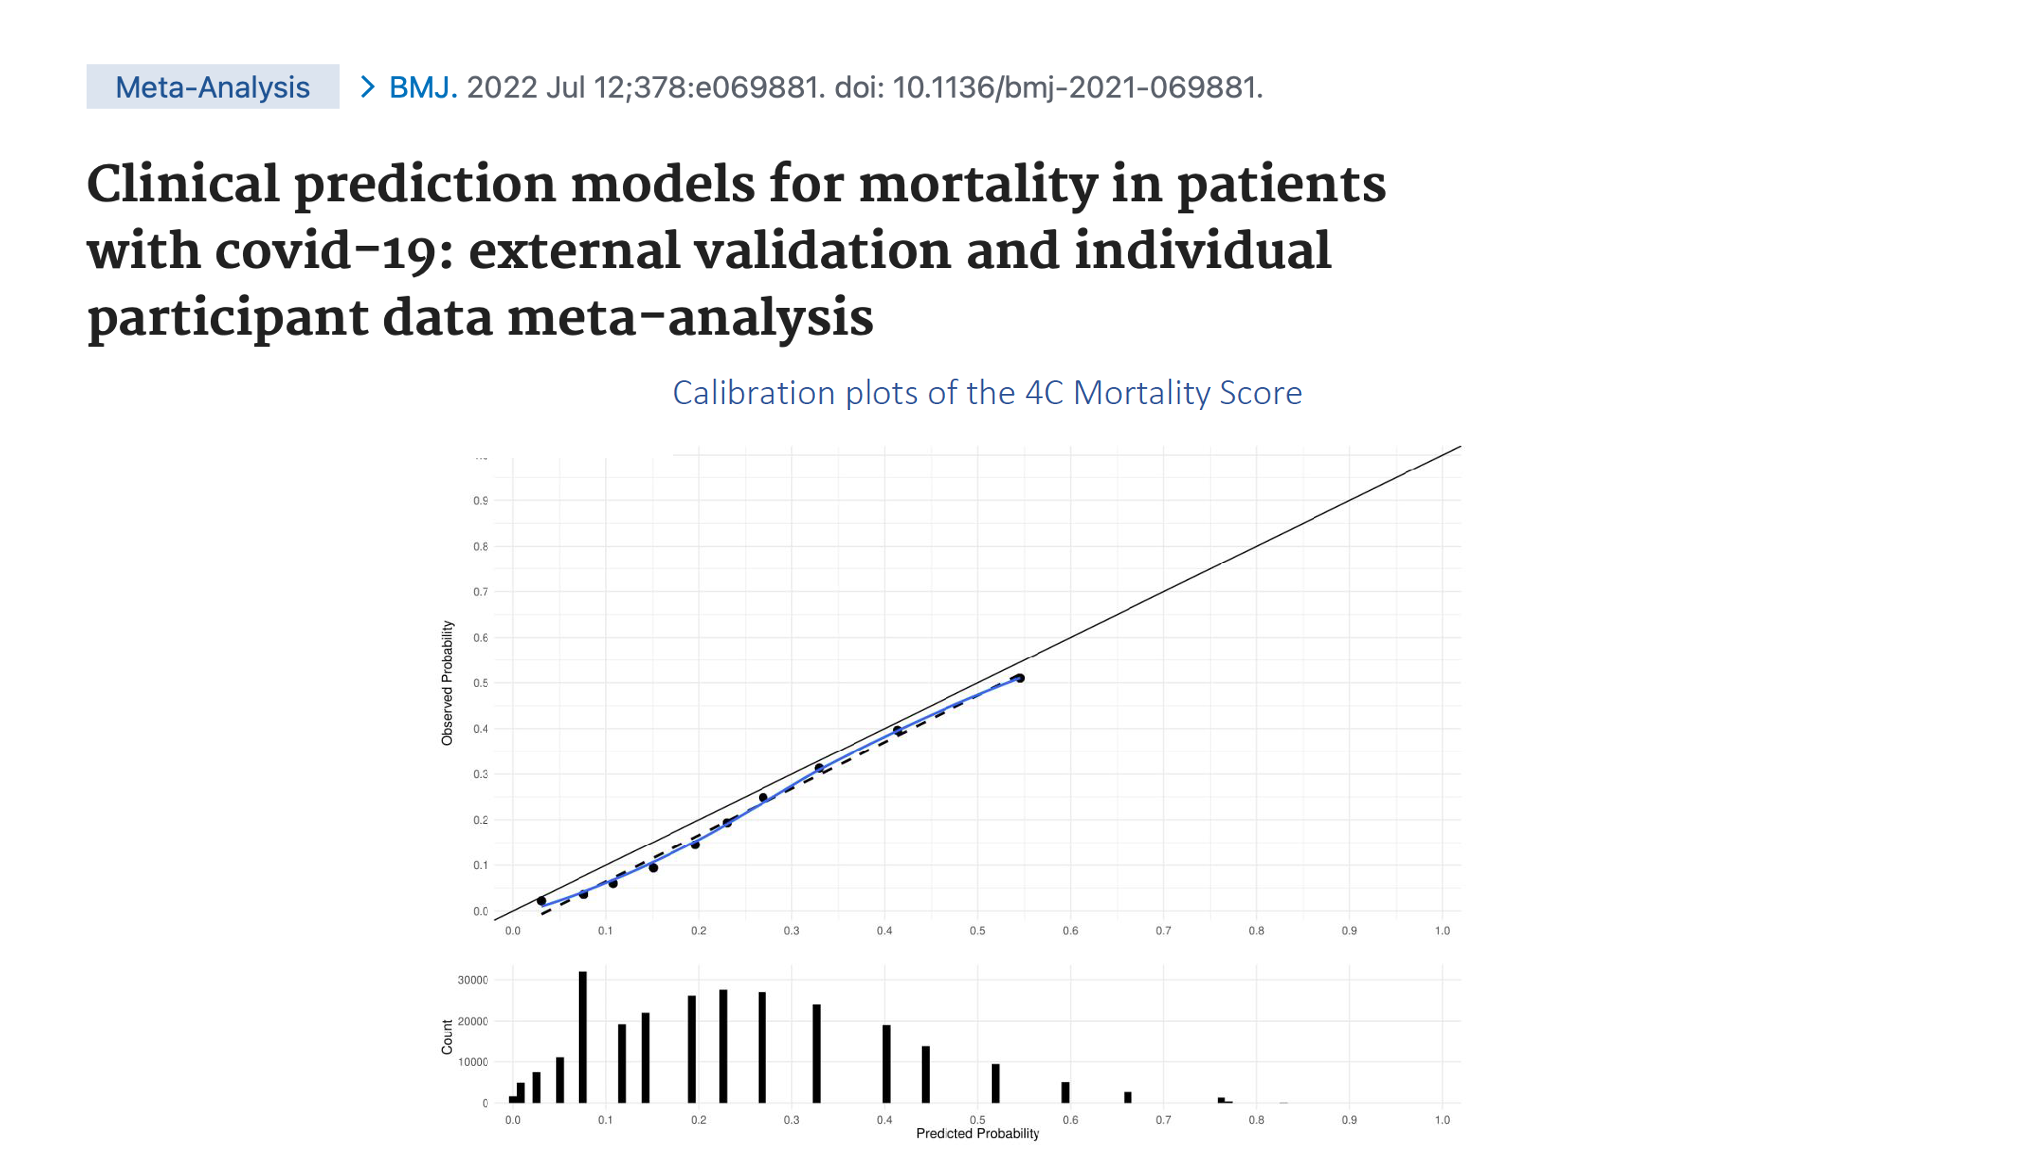
\includegraphics{images/F1.png}

\begin{center}\rule{0.5\linewidth}{0.5pt}\end{center}

{ Calibration plots from clusters}

\begin{Shaded}
\begin{Highlighting}[]
\FunctionTok{ggplot}\NormalTok{(}\AttributeTok{data =}\NormalTok{ dataplot, }\FunctionTok{aes}\NormalTok{(}\AttributeTok{x =}\NormalTok{ pi, }\AttributeTok{y =}\NormalTok{pr,}\AttributeTok{color=}\FunctionTok{as.factor}\NormalTok{(cluster))) }\SpecialCharTok{+}
  \FunctionTok{theme\_light}\NormalTok{()}\SpecialCharTok{+}
  \FunctionTok{geom\_ribbon}\NormalTok{(}\FunctionTok{aes}\NormalTok{(}\AttributeTok{ymin =}\NormalTok{ Lpr, }\AttributeTok{ymax =}\NormalTok{ Upr), }\AttributeTok{fill =} \StringTok{"lightgray"}\NormalTok{,}\AttributeTok{alpha =}\NormalTok{ .}\DecValTok{3}\NormalTok{, }\AttributeTok{colour =} \ConstantTok{NA}\NormalTok{)}\SpecialCharTok{+} 
  \FunctionTok{geom\_abline}\NormalTok{(}\AttributeTok{color=}\StringTok{"black"}\NormalTok{,}\AttributeTok{linetype=}\StringTok{"dashed"}\NormalTok{)}\SpecialCharTok{+}
  \FunctionTok{geom\_line}\NormalTok{(}\AttributeTok{color=}\StringTok{"\#047C90"}\NormalTok{)}\SpecialCharTok{+}
  \FunctionTok{facet\_wrap}\NormalTok{(}\SpecialCharTok{\textasciitilde{}}\NormalTok{cluster,}\AttributeTok{ncol=}\DecValTok{10}\NormalTok{)}\SpecialCharTok{+}
  \FunctionTok{labs}\NormalTok{( }\AttributeTok{x =}\FunctionTok{expression}\NormalTok{(}\StringTok{"Estimated probability"}\SpecialCharTok{\textasciitilde{}}\NormalTok{(pi)),}
        \AttributeTok{y =} \StringTok{"Empirical probability"}\NormalTok{)}\SpecialCharTok{+}
  \FunctionTok{theme}\NormalTok{(}\AttributeTok{legend.position=}\StringTok{"none"}\NormalTok{)}\SpecialCharTok{+}
  \FunctionTok{theme}\NormalTok{(}\AttributeTok{axis.text.x =} \FunctionTok{element\_text}\NormalTok{(}\AttributeTok{angle =} \DecValTok{45}\NormalTok{, }\AttributeTok{vjust =} \FloatTok{0.5}\NormalTok{, }\AttributeTok{hjust=}\DecValTok{1}\NormalTok{))}
\end{Highlighting}
\end{Shaded}

\begin{figure}[H]

{\centering 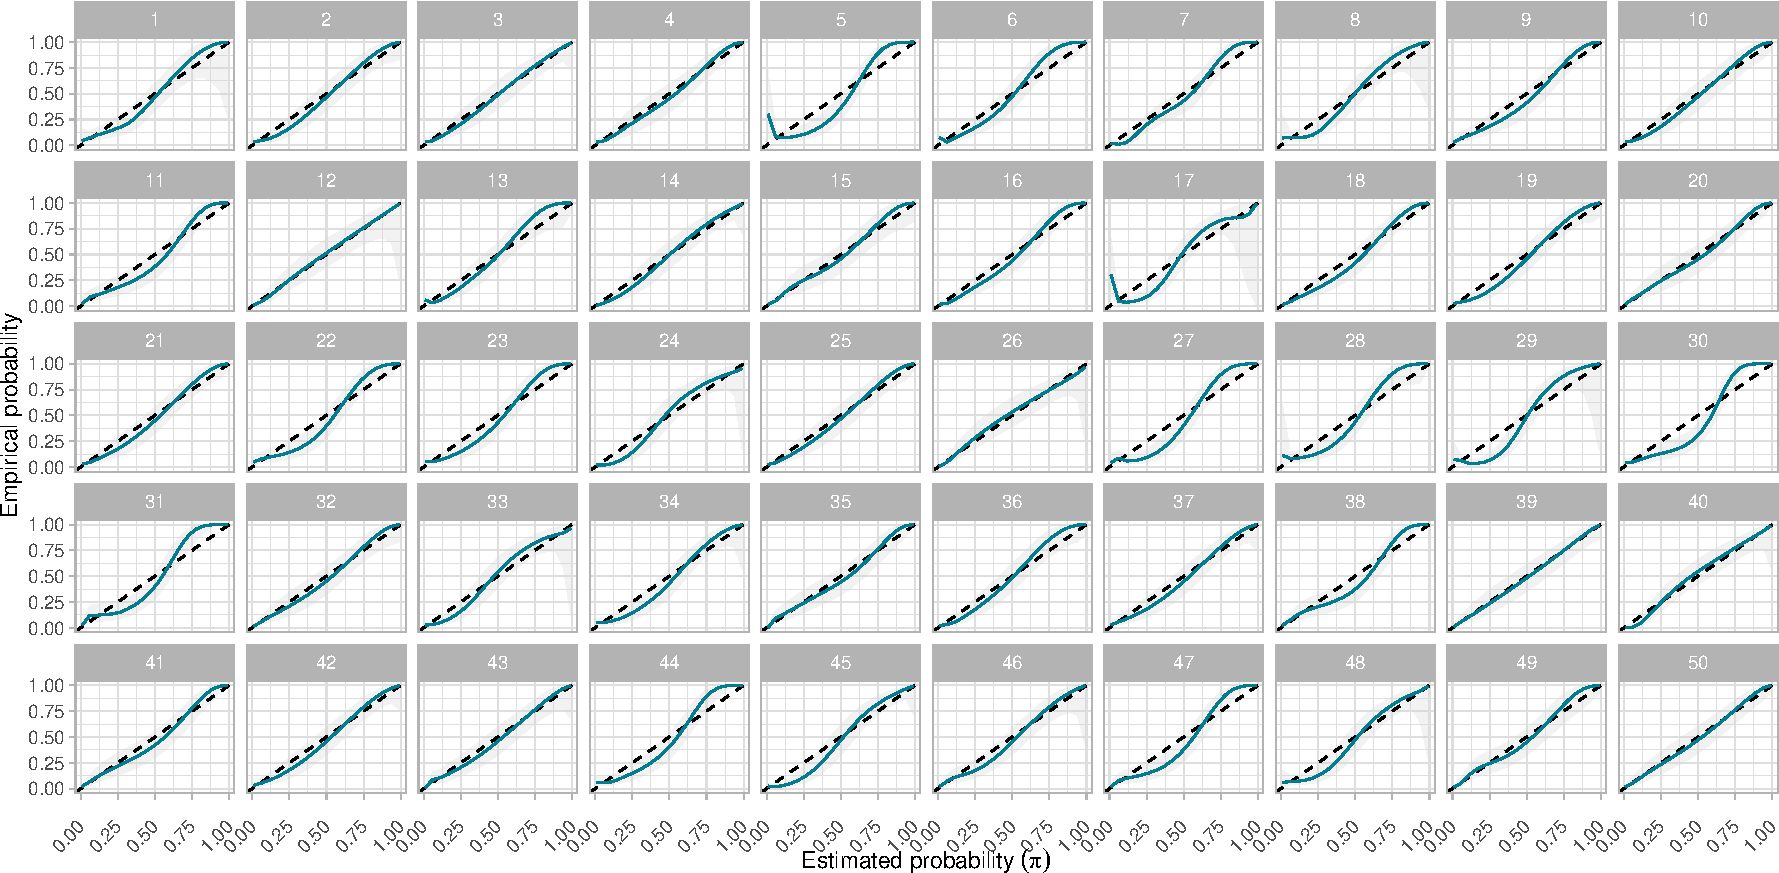
\includegraphics{index_files/figure-pdf/unnamed-chunk-2-1.pdf}

}

\end{figure}

\begin{center}\rule{0.5\linewidth}{0.5pt}\end{center}

{ Calibration plots from clusters}

\begin{Shaded}
\begin{Highlighting}[]
\FunctionTok{ggplot}\NormalTok{(}\AttributeTok{data =}\NormalTok{ dataplot) }\SpecialCharTok{+}
  \FunctionTok{theme\_light}\NormalTok{()}\SpecialCharTok{+}
  \FunctionTok{geom\_line}\NormalTok{(}\FunctionTok{aes}\NormalTok{(}\AttributeTok{x =}\NormalTok{ pi, }\AttributeTok{y =}\NormalTok{ pr,}\AttributeTok{group=}\NormalTok{cluster),}\AttributeTok{color=}\StringTok{"\#047C90"}\NormalTok{,}\AttributeTok{alpha=}\FloatTok{0.2}\NormalTok{)}\SpecialCharTok{+}
  \FunctionTok{labs}\NormalTok{( }\AttributeTok{x =}\FunctionTok{expression}\NormalTok{(}\StringTok{"Estimated probability"}\SpecialCharTok{\textasciitilde{}}\NormalTok{(pi)),}
        \AttributeTok{y =} \StringTok{"Actual proportion"}\NormalTok{)}\SpecialCharTok{+}
  \FunctionTok{theme}\NormalTok{(}\AttributeTok{legend.position=}\StringTok{"none"}\NormalTok{)}\SpecialCharTok{+}
  \FunctionTok{geom\_line}\NormalTok{(}\AttributeTok{data=}\NormalTok{sdata,}\FunctionTok{aes}\NormalTok{(x,y),}\AttributeTok{size=}\FloatTok{1.5}\NormalTok{,}\AttributeTok{color=}\StringTok{"\#003660"}\NormalTok{)}\SpecialCharTok{+}
  \FunctionTok{geom\_abline}\NormalTok{(}\AttributeTok{color=}\StringTok{"black"}\NormalTok{,}\AttributeTok{linetype=}\StringTok{"dashed"}\NormalTok{)}\SpecialCharTok{+}
   \FunctionTok{labs}\NormalTok{( }\AttributeTok{x =}\FunctionTok{expression}\NormalTok{(}\StringTok{"Estimated probability"}\SpecialCharTok{\textasciitilde{}}\NormalTok{(pi)),}
        \AttributeTok{y =} \StringTok{"Empirical probability"}\NormalTok{)}\SpecialCharTok{+}
  \FunctionTok{theme}\NormalTok{(}\AttributeTok{legend.position=}\StringTok{"none"}\NormalTok{)}
\end{Highlighting}
\end{Shaded}

\begin{verbatim}
Warning: Using `size` aesthetic for lines was deprecated in ggplot2 3.4.0.
i Please use `linewidth` instead.
\end{verbatim}

\begin{figure}[H]

{\centering 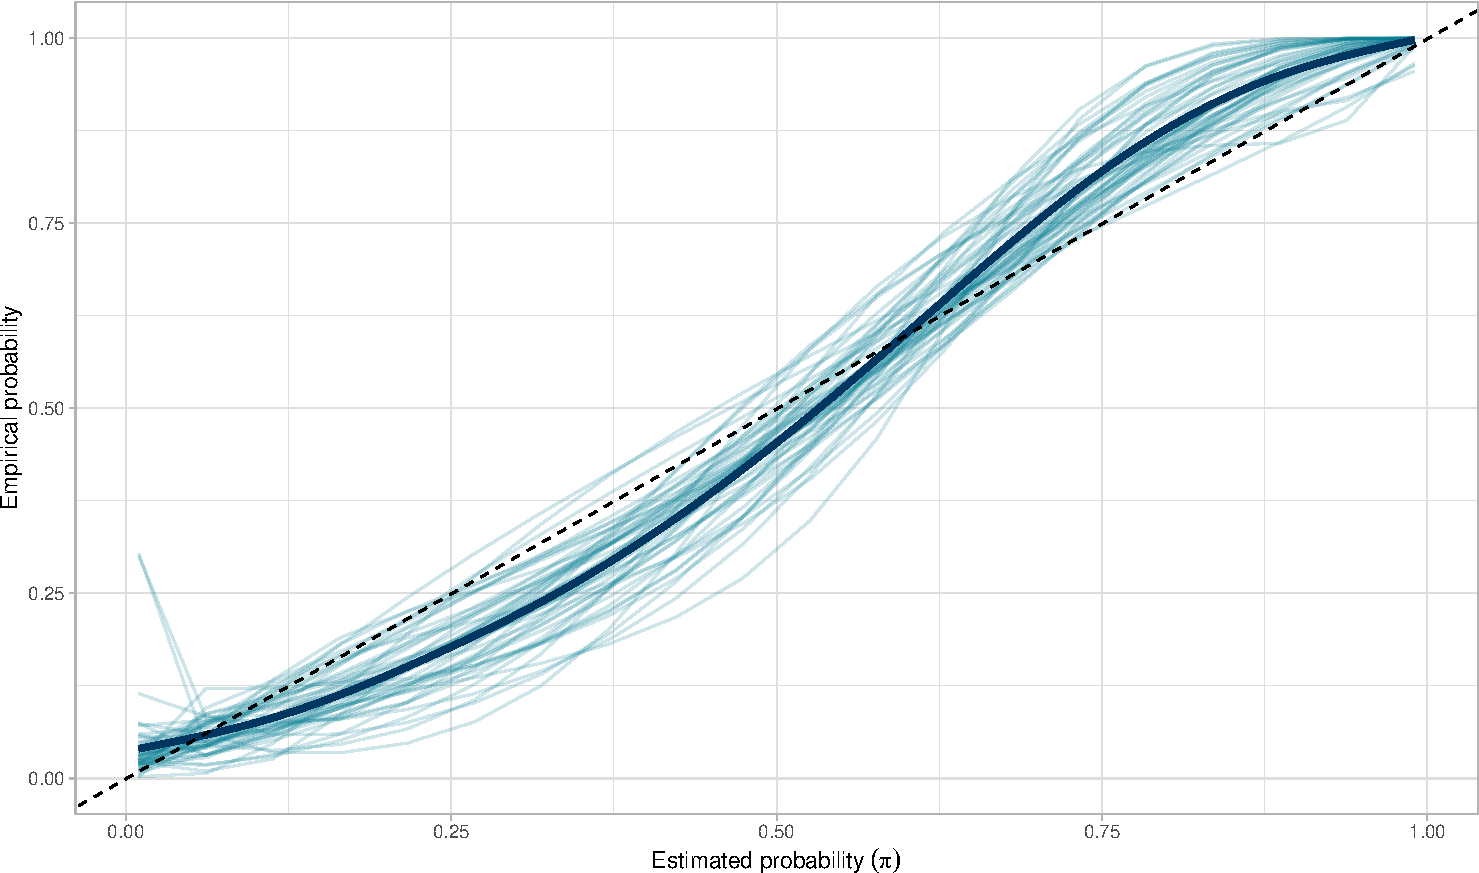
\includegraphics{index_files/figure-pdf/unnamed-chunk-3-1.pdf}

}

\end{figure}

\begin{center}\rule{0.5\linewidth}{0.5pt}\end{center}

{ Calibration plots from clusters}

\begin{Shaded}
\begin{Highlighting}[]
\FunctionTok{ggplot}\NormalTok{(}\AttributeTok{data =}\NormalTok{ dataplot) }\SpecialCharTok{+}
  \FunctionTok{theme\_light}\NormalTok{()}\SpecialCharTok{+}
    \FunctionTok{geom\_line}\NormalTok{(}\FunctionTok{aes}\NormalTok{(}\AttributeTok{x =}\NormalTok{ pi, }\AttributeTok{y =}\NormalTok{ pr,}\AttributeTok{group=}\NormalTok{cluster),}\AttributeTok{color=}\StringTok{"\#047C90"}\NormalTok{,}\AttributeTok{alpha=}\FloatTok{0.2}\NormalTok{)}\SpecialCharTok{+}
  \FunctionTok{labs}\NormalTok{( }\AttributeTok{x =}\FunctionTok{expression}\NormalTok{(}\StringTok{"Estimated probability"}\SpecialCharTok{\textasciitilde{}}\NormalTok{(pi)),}
        \AttributeTok{y =} \StringTok{"Actual proportion"}\NormalTok{)}\SpecialCharTok{+}
  \FunctionTok{theme}\NormalTok{(}\AttributeTok{legend.position=}\StringTok{"none"}\NormalTok{)}\SpecialCharTok{+}
  \FunctionTok{geom\_ribbon}\NormalTok{(}\AttributeTok{data=}\NormalTok{sdata,}\FunctionTok{aes}\NormalTok{(}\AttributeTok{x=}\NormalTok{x,}\AttributeTok{ymax=}\NormalTok{ymax,}\AttributeTok{ymin=}\NormalTok{ymin), }\AttributeTok{fill =} \StringTok{"white"}\NormalTok{)}\SpecialCharTok{+}
  \FunctionTok{geom\_line}\NormalTok{(}\AttributeTok{data=}\NormalTok{sdata,}\FunctionTok{aes}\NormalTok{(x,y),}\AttributeTok{size=}\FloatTok{1.5}\NormalTok{,}\AttributeTok{color=}\StringTok{"\#003660"}\NormalTok{)}\SpecialCharTok{+}
  \FunctionTok{geom\_abline}\NormalTok{(}\AttributeTok{color=}\StringTok{"black"}\NormalTok{,}\AttributeTok{linetype=}\StringTok{"dashed"}\NormalTok{)}\SpecialCharTok{+}
   \FunctionTok{labs}\NormalTok{( }\AttributeTok{x =}\FunctionTok{expression}\NormalTok{(}\StringTok{"Estimated probability"}\SpecialCharTok{\textasciitilde{}}\NormalTok{(pi)),}
        \AttributeTok{y =} \StringTok{"Empirical probability"}\NormalTok{)}\SpecialCharTok{+}
  \FunctionTok{theme}\NormalTok{(}\AttributeTok{legend.position=}\StringTok{"none"}\NormalTok{)}
\end{Highlighting}
\end{Shaded}

\begin{figure}[H]

{\centering 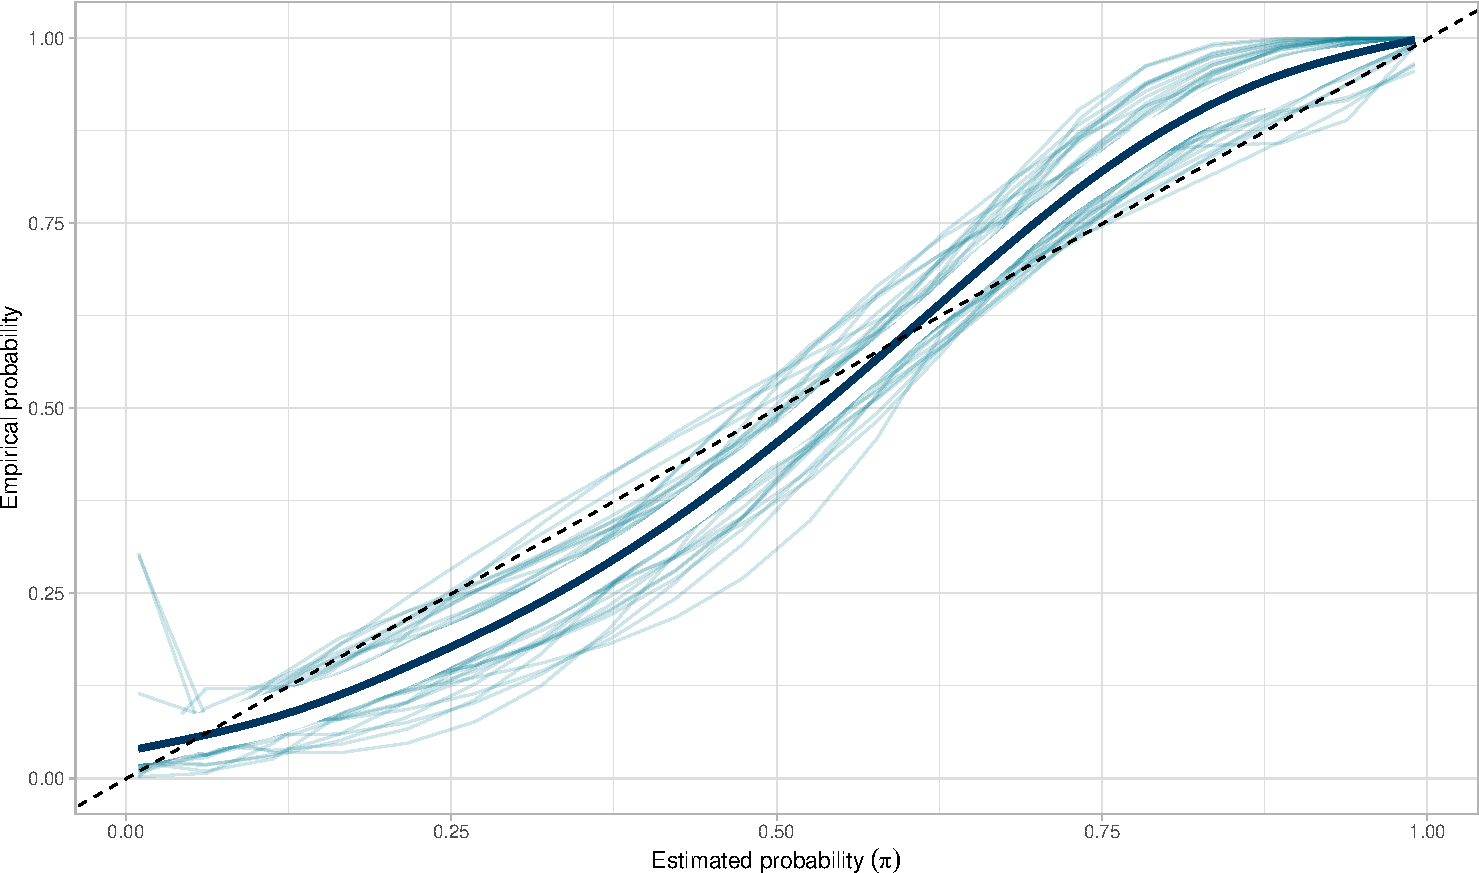
\includegraphics{index_files/figure-pdf/unnamed-chunk-4-1.pdf}

}

\end{figure}

\begin{center}\rule{0.5\linewidth}{0.5pt}\end{center}

{ Multiple Imputation}

\textbf{Aim:} Evaluate methods for synthesizing calibration curves from
multiple imputed datasets in terms of confidence interval (CI) length,
bias and coverage.

We focus on:

\begin{itemize}
\tightlist
\item
  Smoothed calibration curves.
\item
  Smooth functions : Loess, locfit, natural splines.
\item
  Confidence intervals: Closed form, bootstrap.
\end{itemize}

\begin{center}\rule{0.5\linewidth}{0.5pt}\end{center}

{ Data generation}

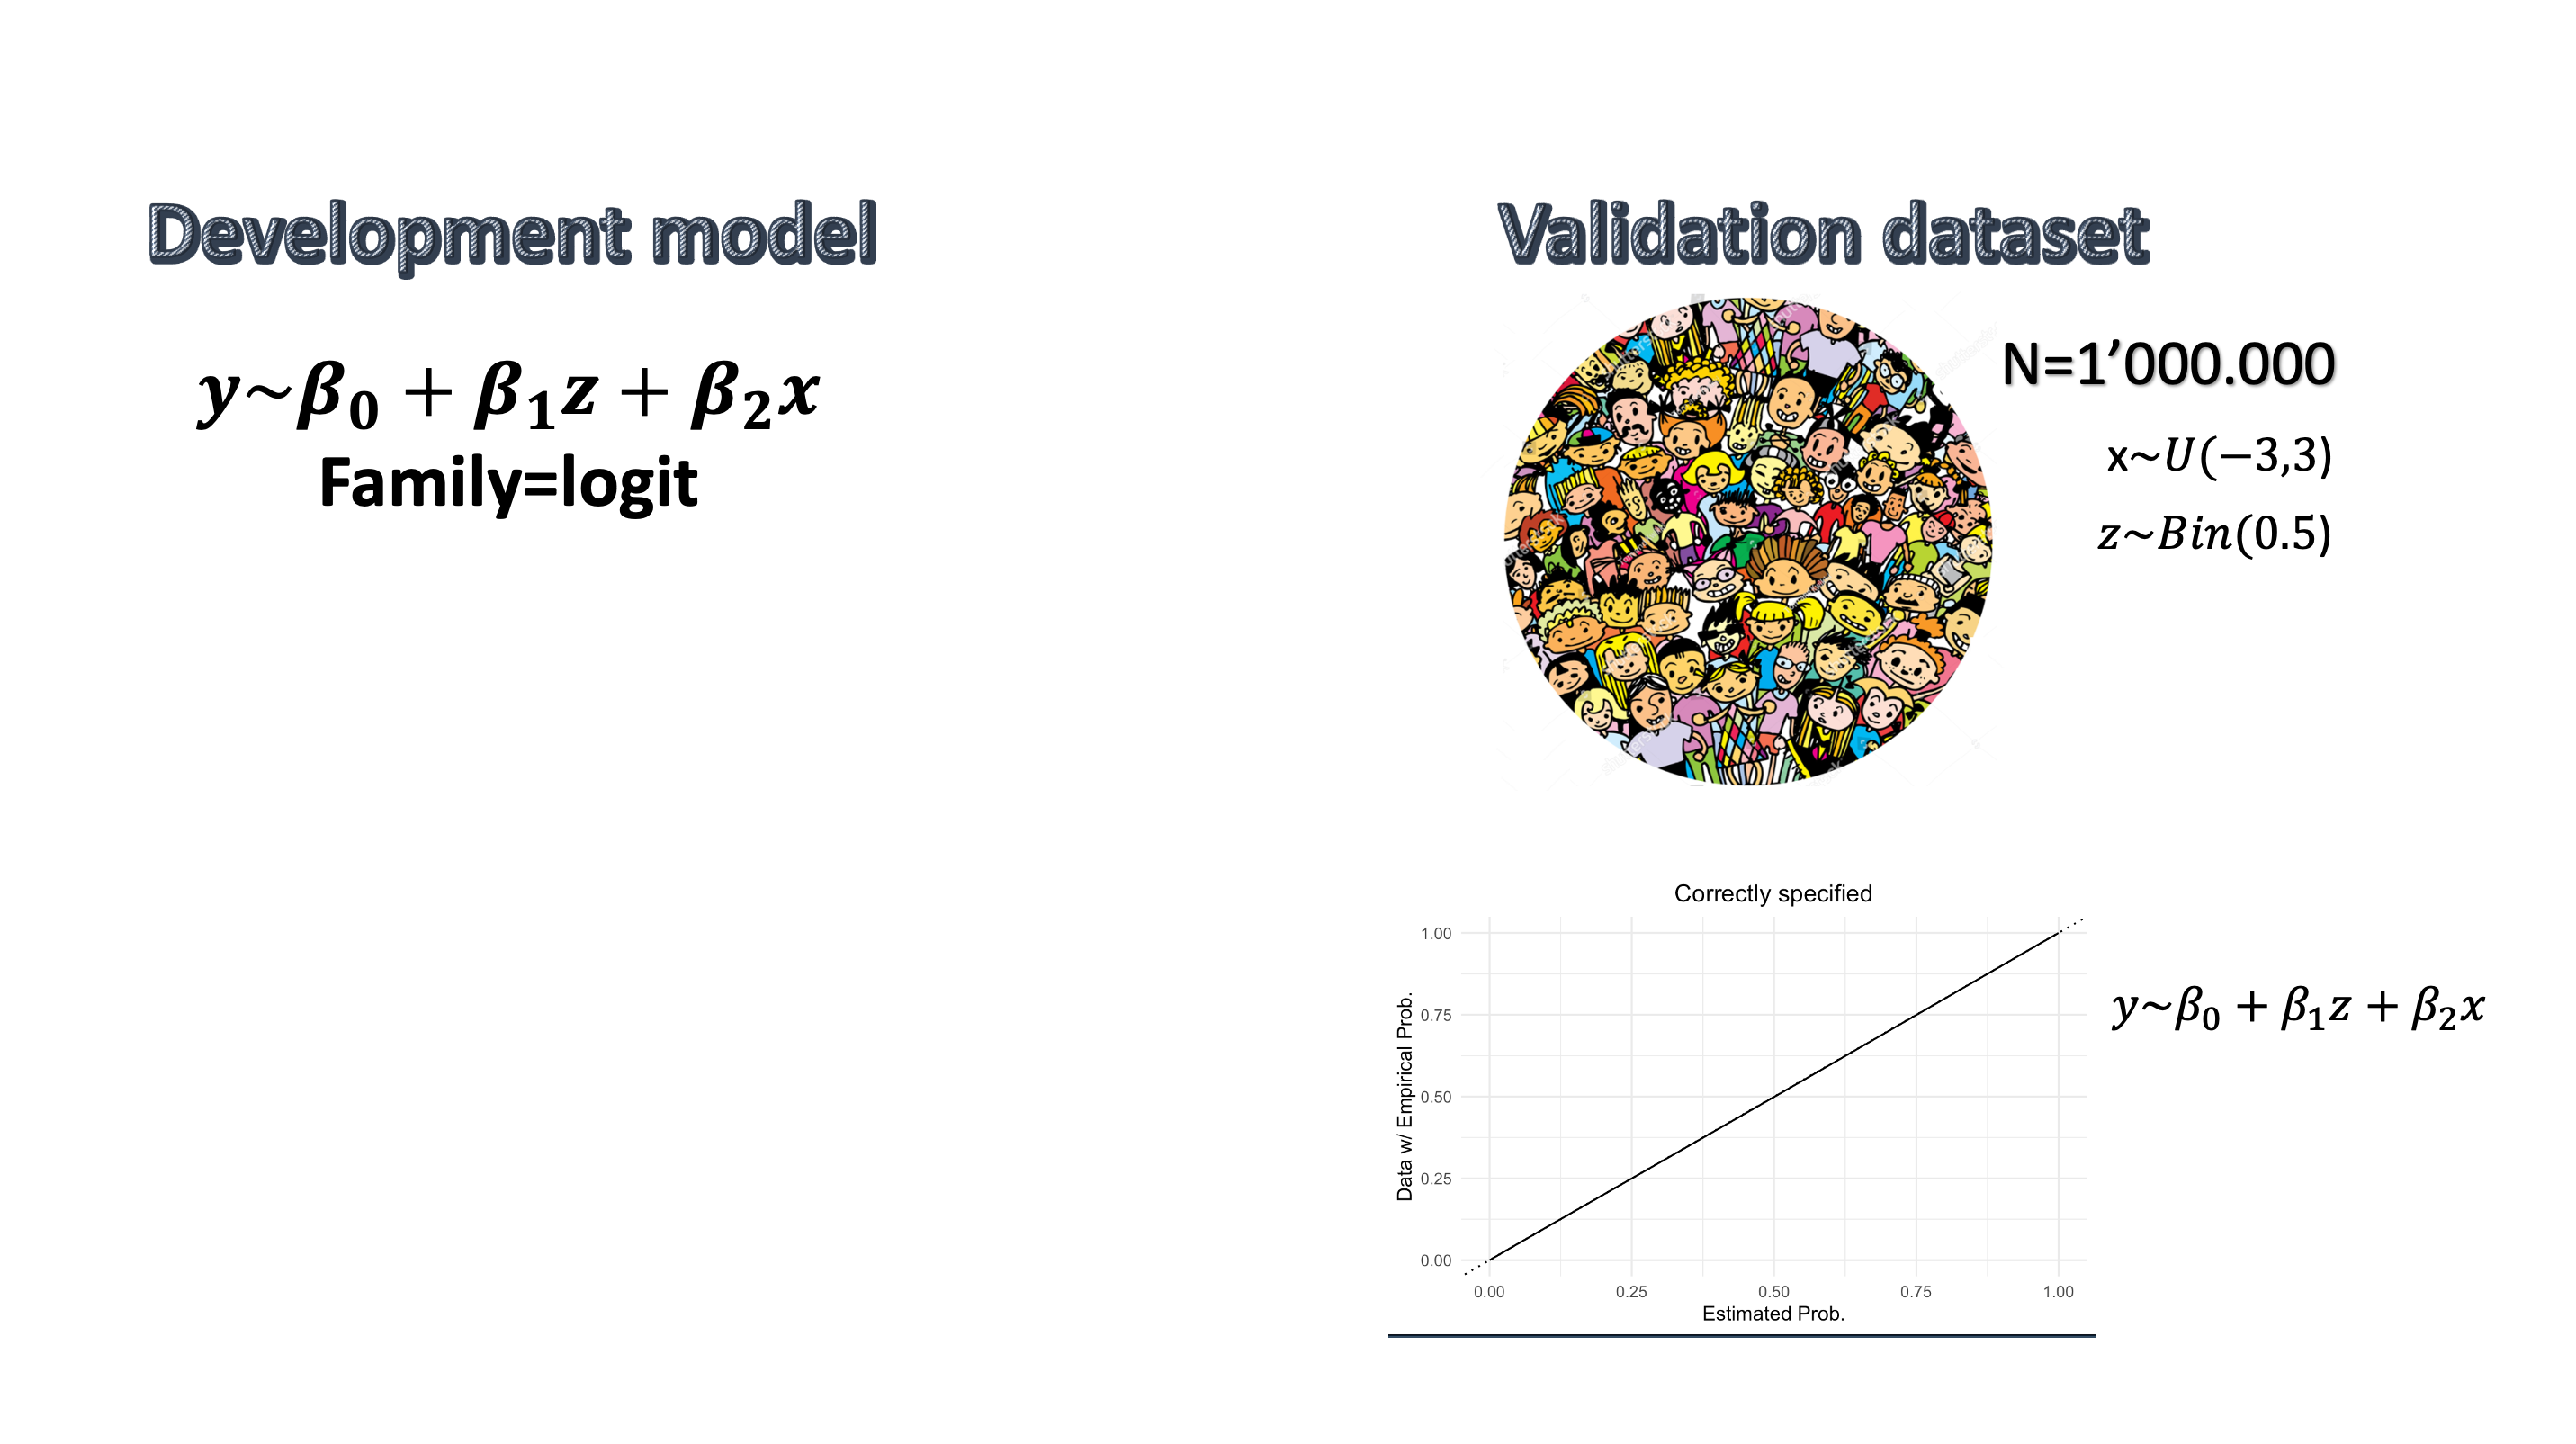
\includegraphics{images/d1.png}

\begin{center}\rule{0.5\linewidth}{0.5pt}\end{center}

{ Data generation}

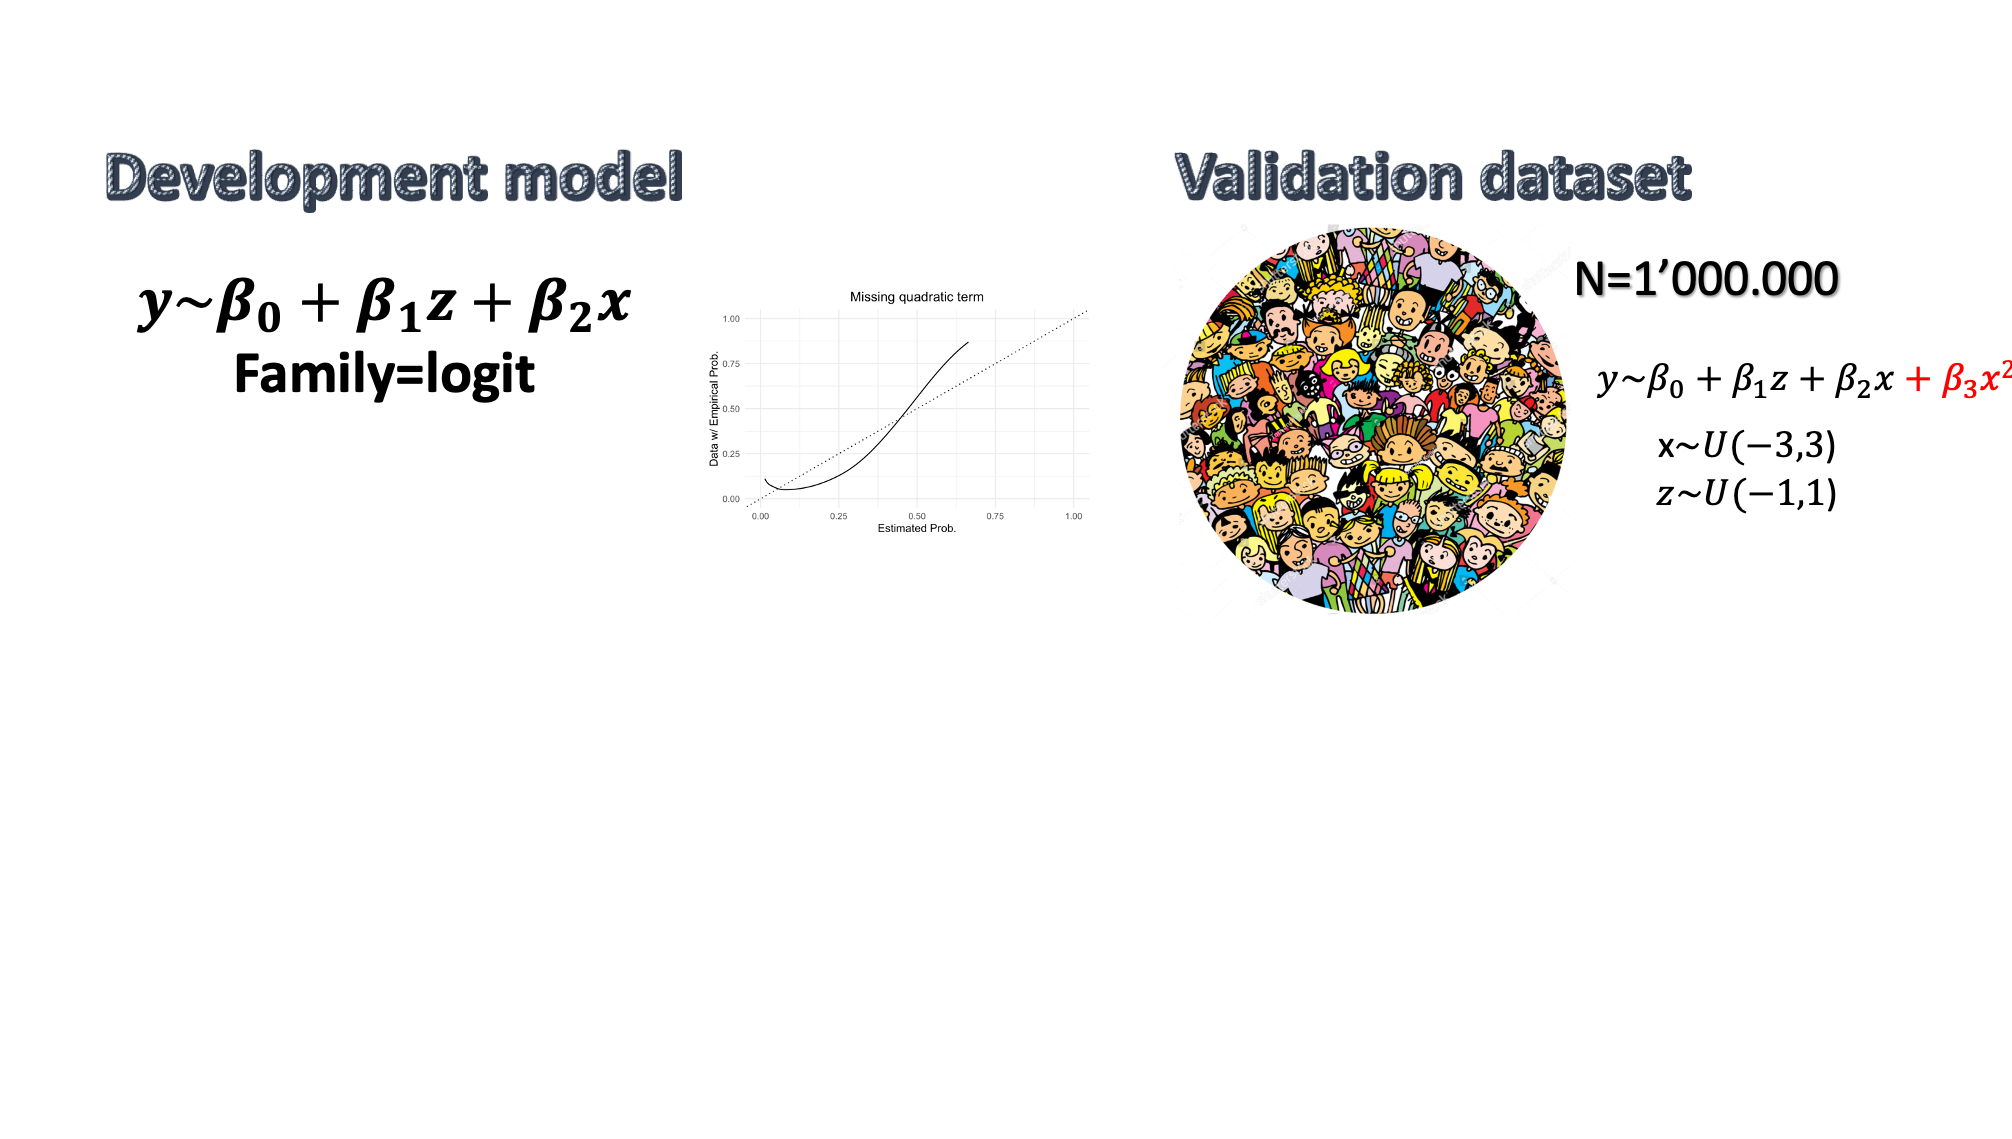
\includegraphics{images/d2.png}

\begin{center}\rule{0.5\linewidth}{0.5pt}\end{center}

{ Data generation}

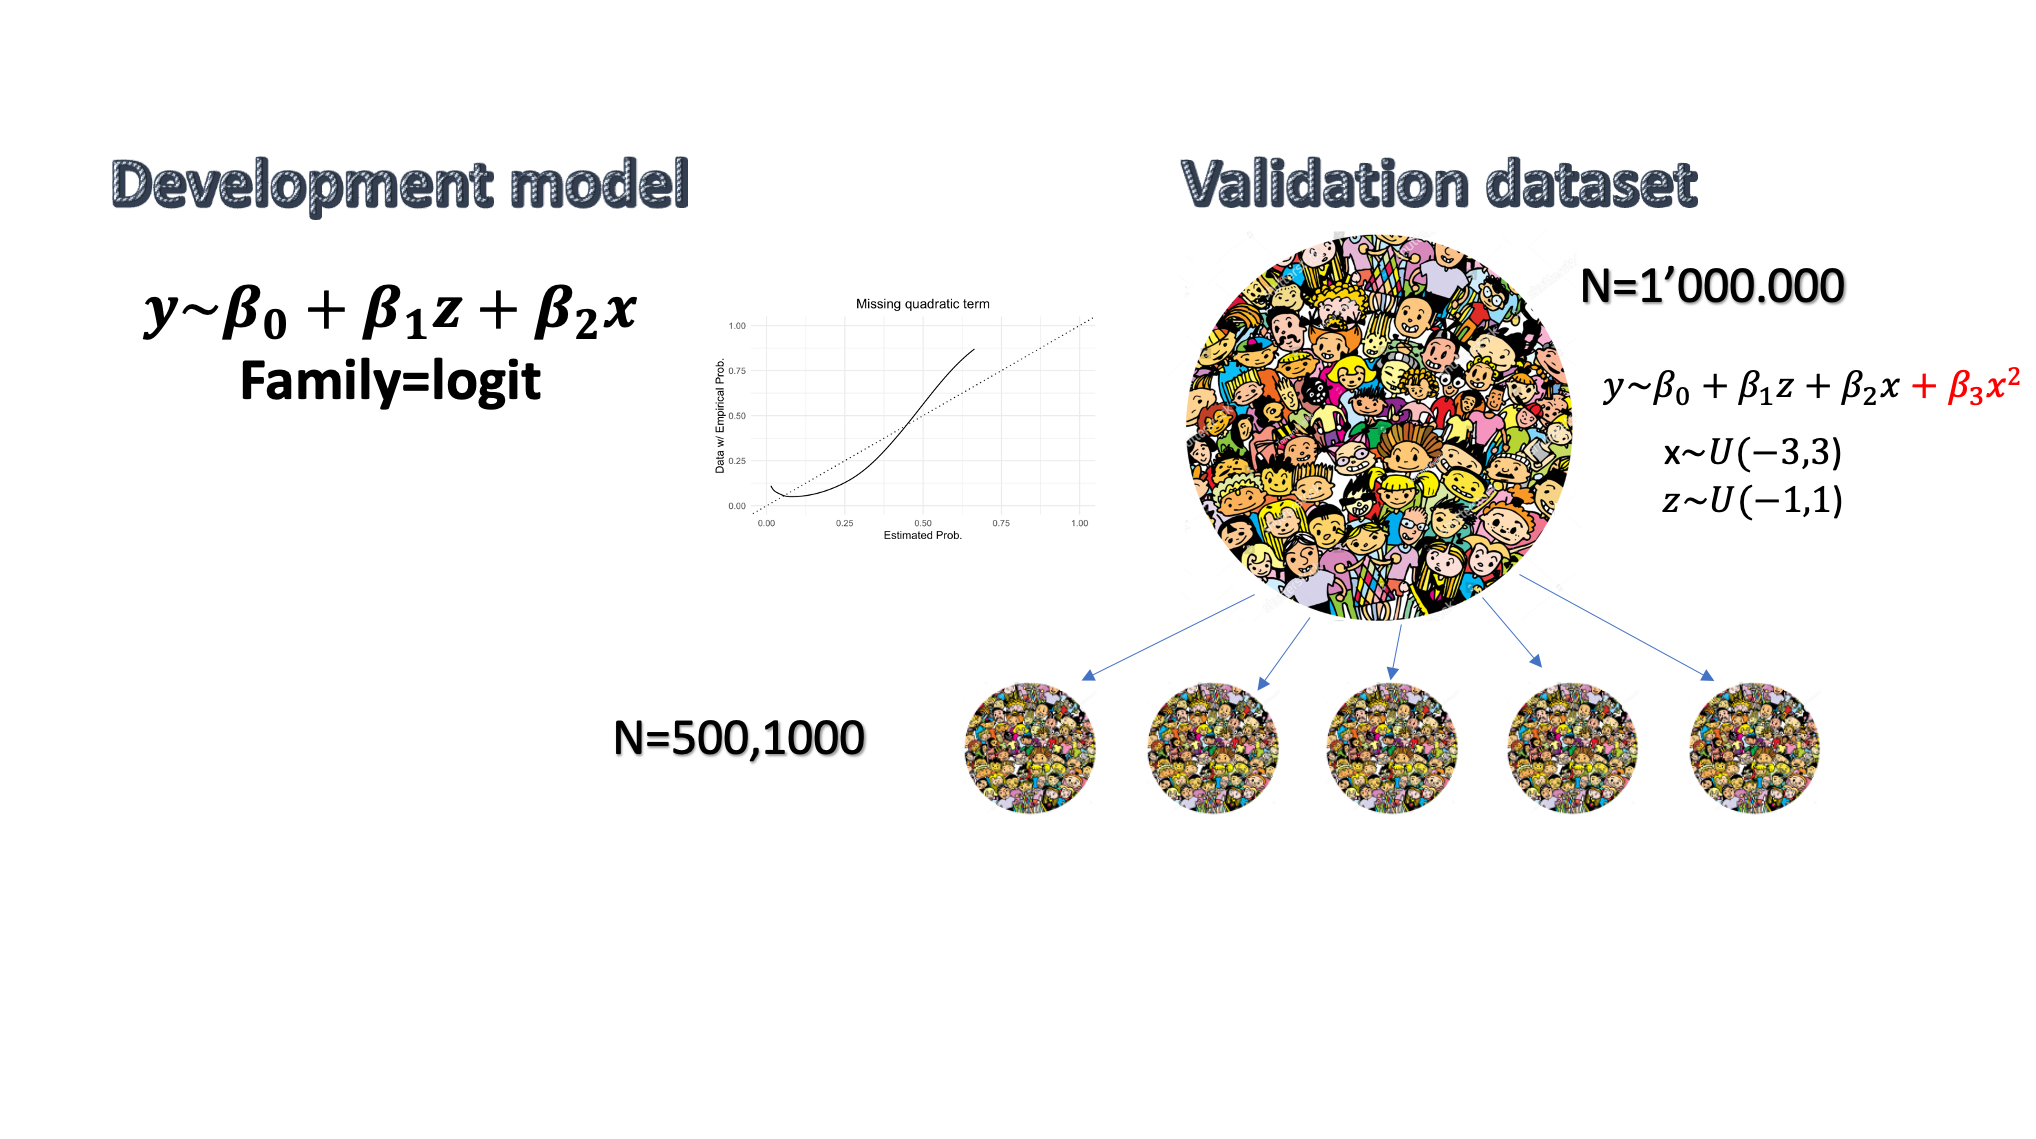
\includegraphics{images/d3.png}

\begin{center}\rule{0.5\linewidth}{0.5pt}\end{center}

{ Data generation}

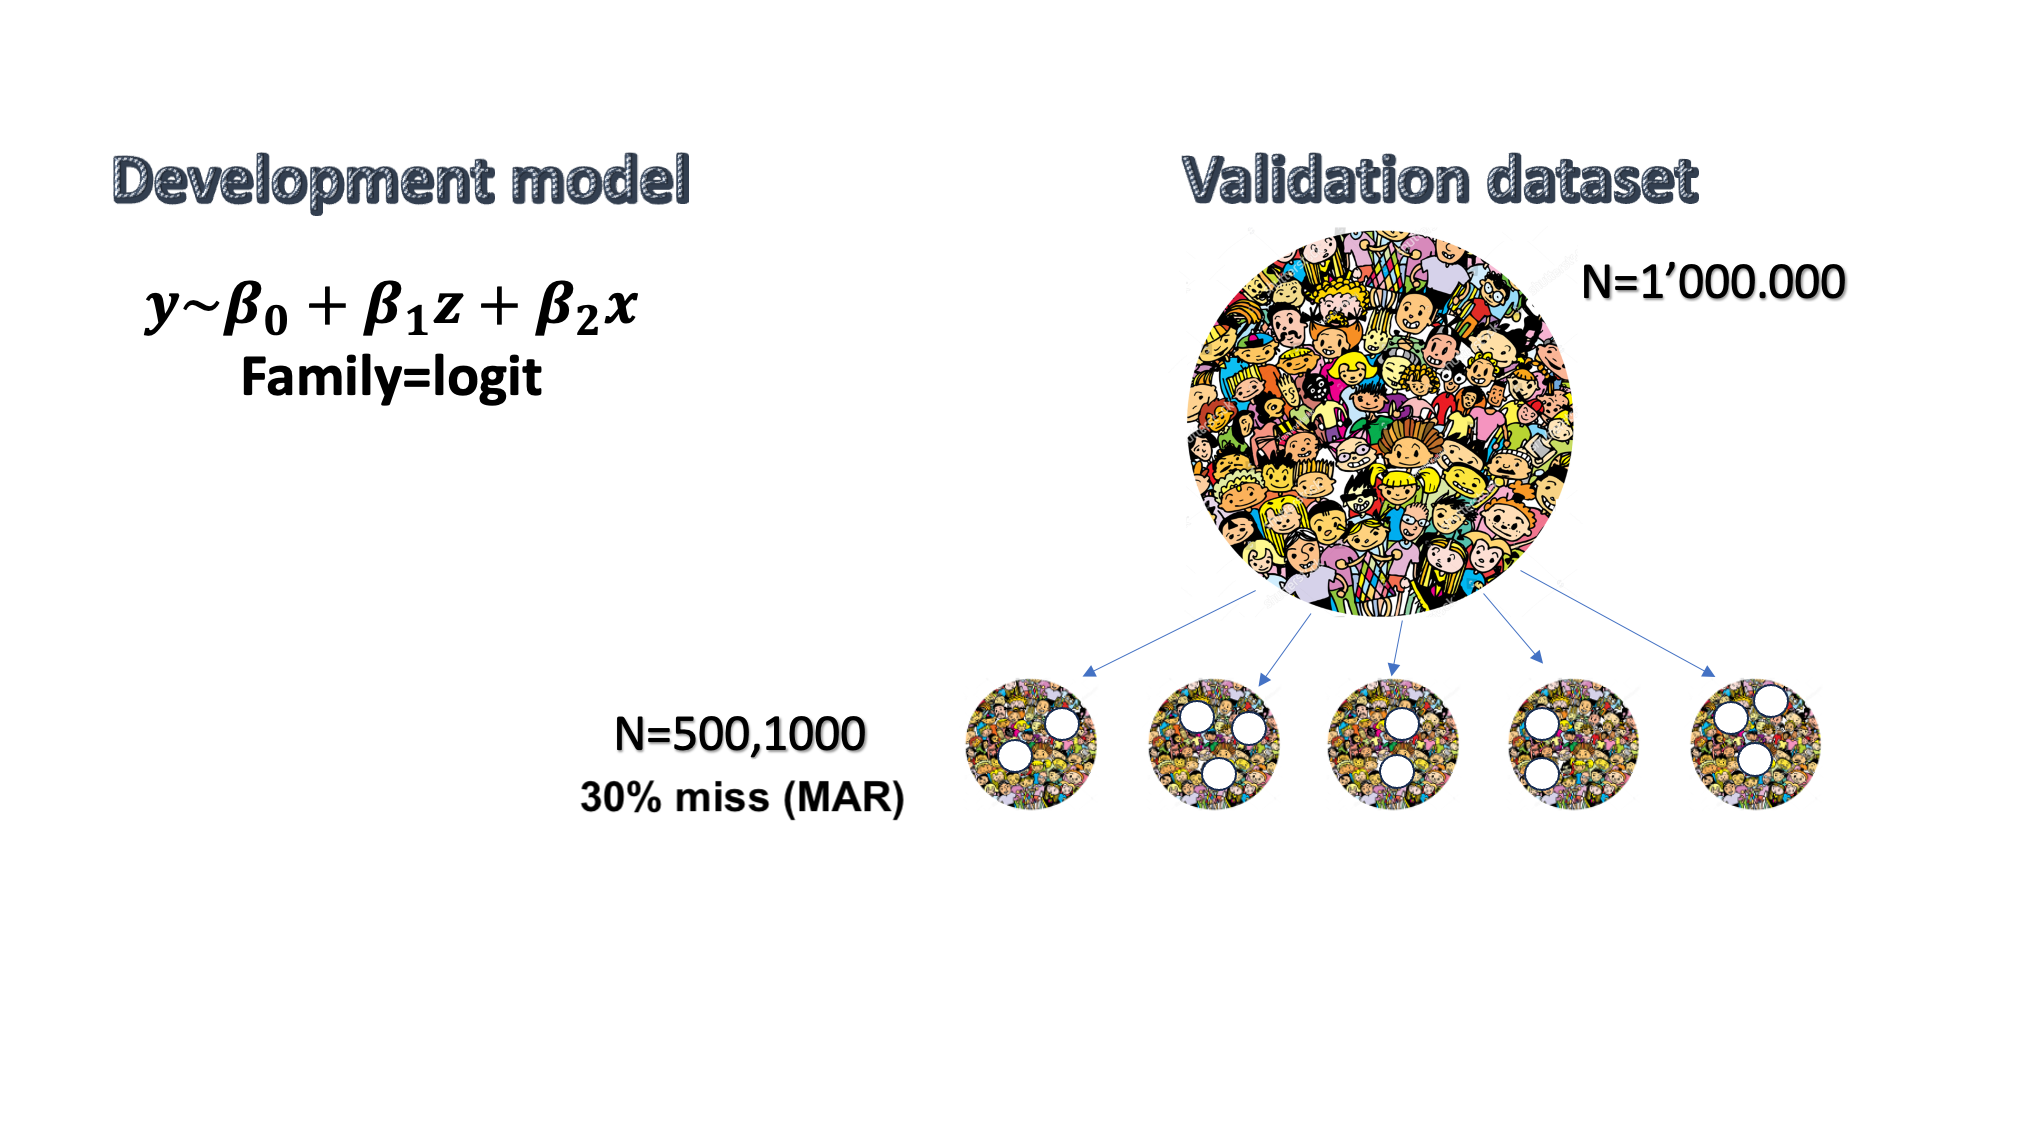
\includegraphics{images/d4.png}

\begin{center}\rule{0.5\linewidth}{0.5pt}\end{center}

{ Data generation}

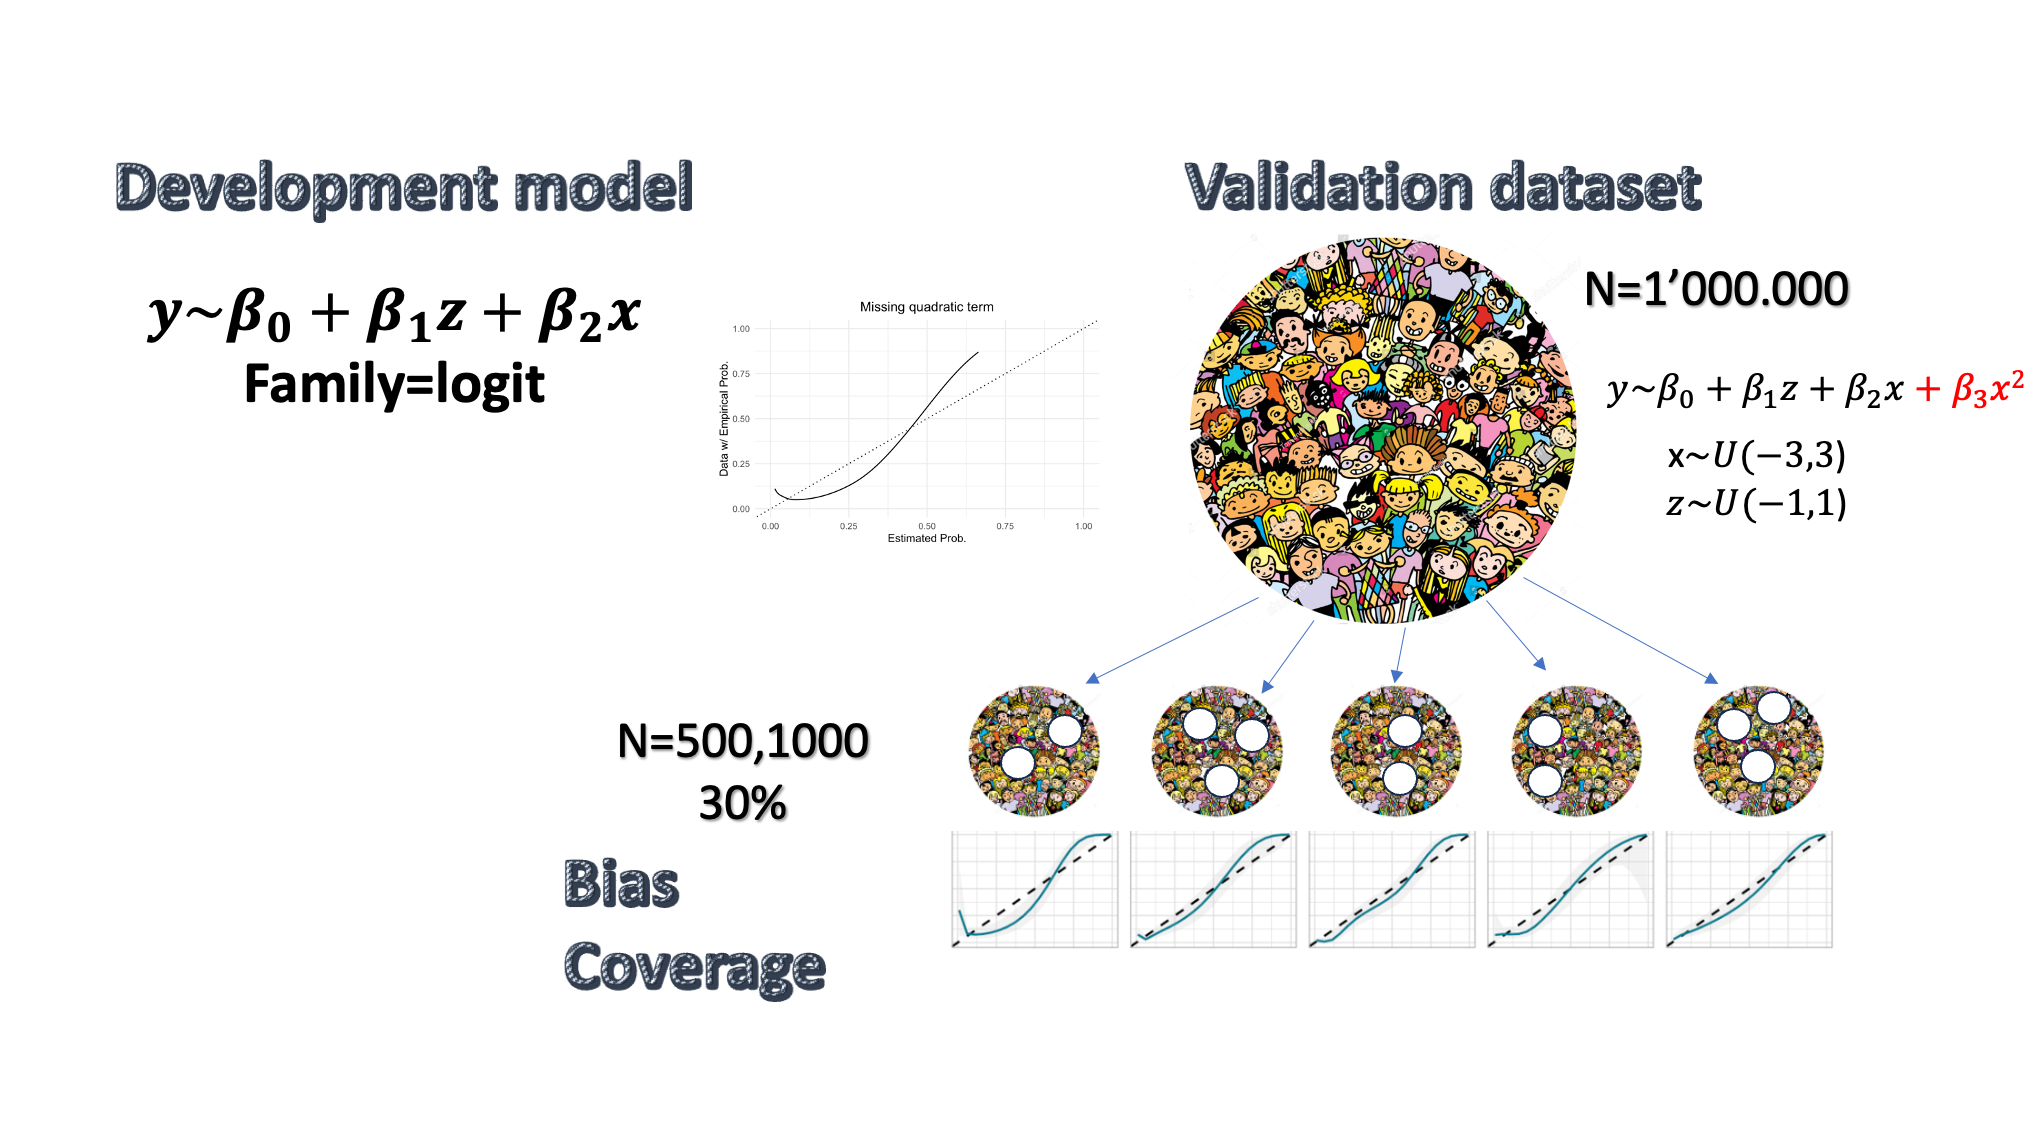
\includegraphics{images/d5.png}

\begin{center}\rule{0.5\linewidth}{0.5pt}\end{center}

{ Methods}

\textbf{1. Multiple imputation only (m):}

{ MI = 10.}

\begin{itemize}
\item
  \textbf{m\_stack:} Stack imputed datasets.
\item
  \textbf{m\_RRPar:} Calibration model with pooled parameters.
\item
  \textbf{m\_RR:} Pooled closed form SE with Rubin Rules.
\end{itemize}

\begin{center}\rule{0.5\linewidth}{0.5pt}\end{center}

{ Methods}

\textbf{2. MICE followed by bootstrap (mb):}

{ BS = 1000, MI = 10.}

\begin{itemize}
\item
  \textbf{mb\_Qp:} Bootstrap percentile pooled sample.
\item
  \textbf{mb\_RR:} Pooled with Rubin's rules.
\end{itemize}

\begin{center}\rule{0.5\linewidth}{0.5pt}\end{center}

{ Methods}

\textbf{3. Bootstrap followed by MICE (bm):}

{ BS = 1000.}

\begin{itemize}
\item
  \textbf{bm\_Q:} Bootstrap percentile (M=10).
\item
  \textbf{bm\_Qp:} Bootstrap percentile pooled sample (M=10).
\item
  \textbf{bm\_VH:} von Hippel and Bartlett (M=2).
\item
  \textbf{bm\_Q1:} Single imputation (M=1).
\end{itemize}

\begin{center}\rule{0.5\linewidth}{0.5pt}\end{center}

{ Conditional results} 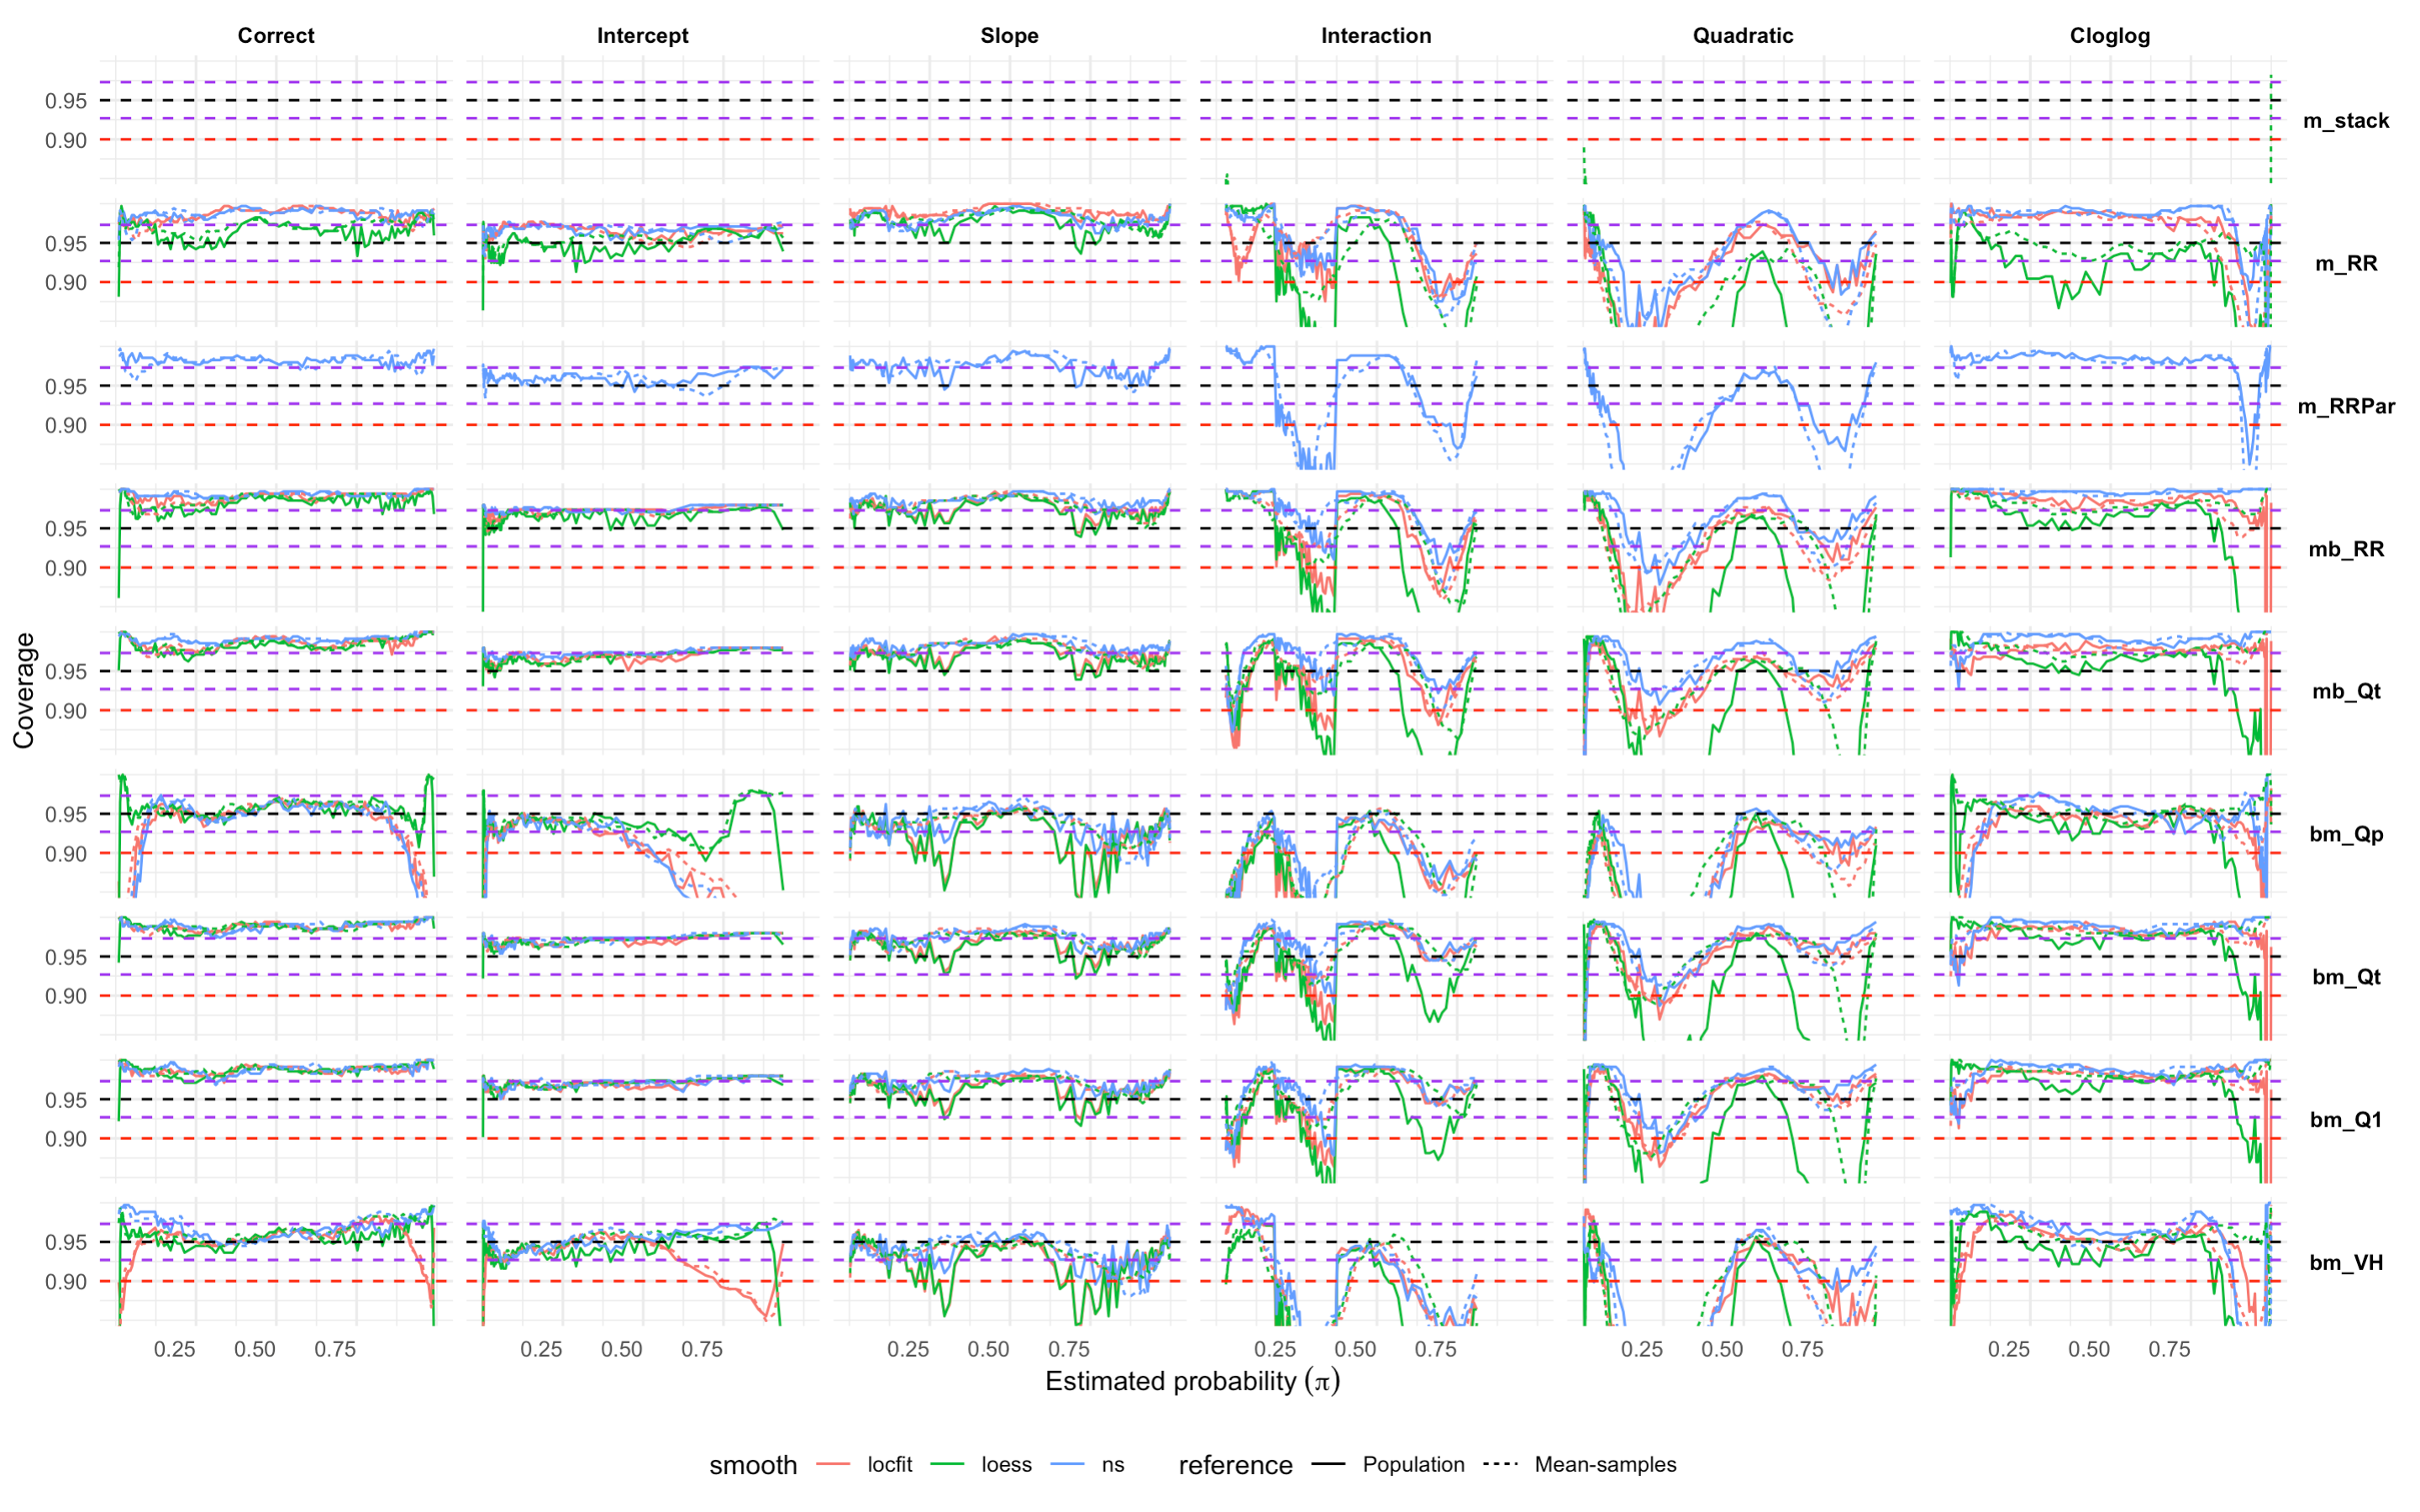
\includegraphics{images/Cond.png}

\begin{center}\rule{0.5\linewidth}{0.5pt}\end{center}

{ Marginal results: CI length} \includegraphics{images/ci500.png}

\begin{center}\rule{0.5\linewidth}{0.5pt}\end{center}

{ Marginal results: Bias} 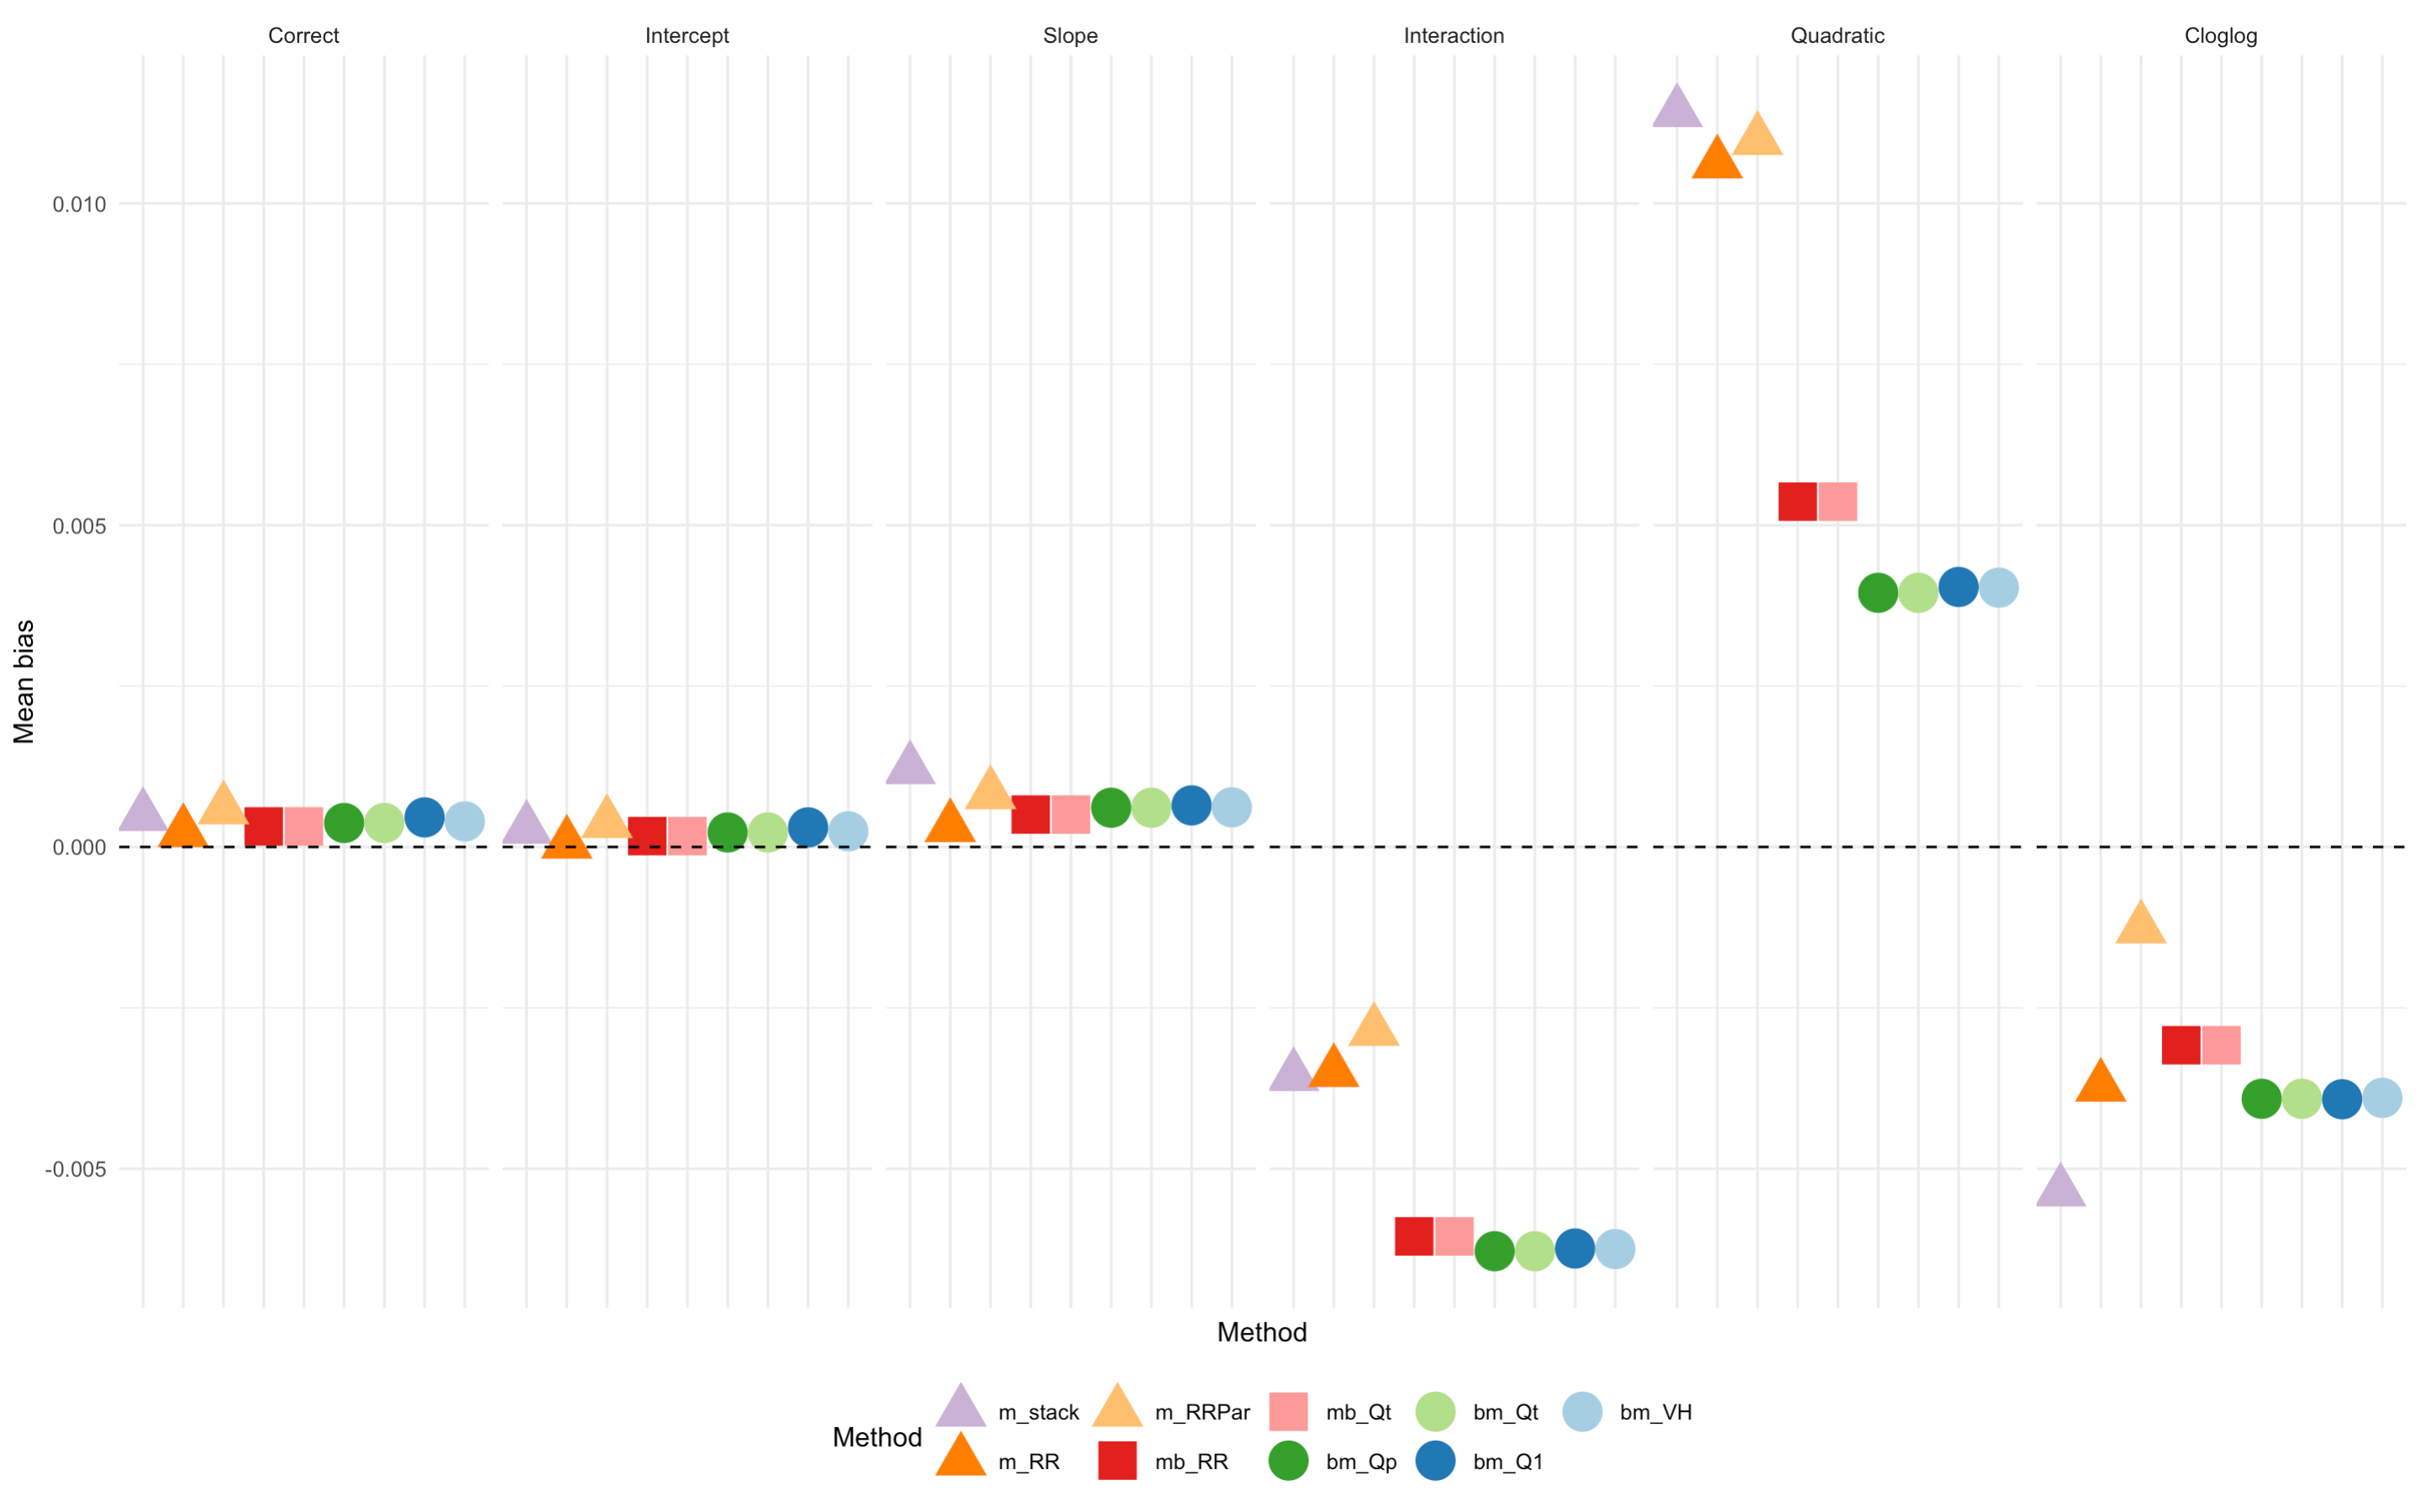
\includegraphics{images/meanbias.png}

\begin{center}\rule{0.5\linewidth}{0.5pt}\end{center}

{ Best method : Mean absolute error}
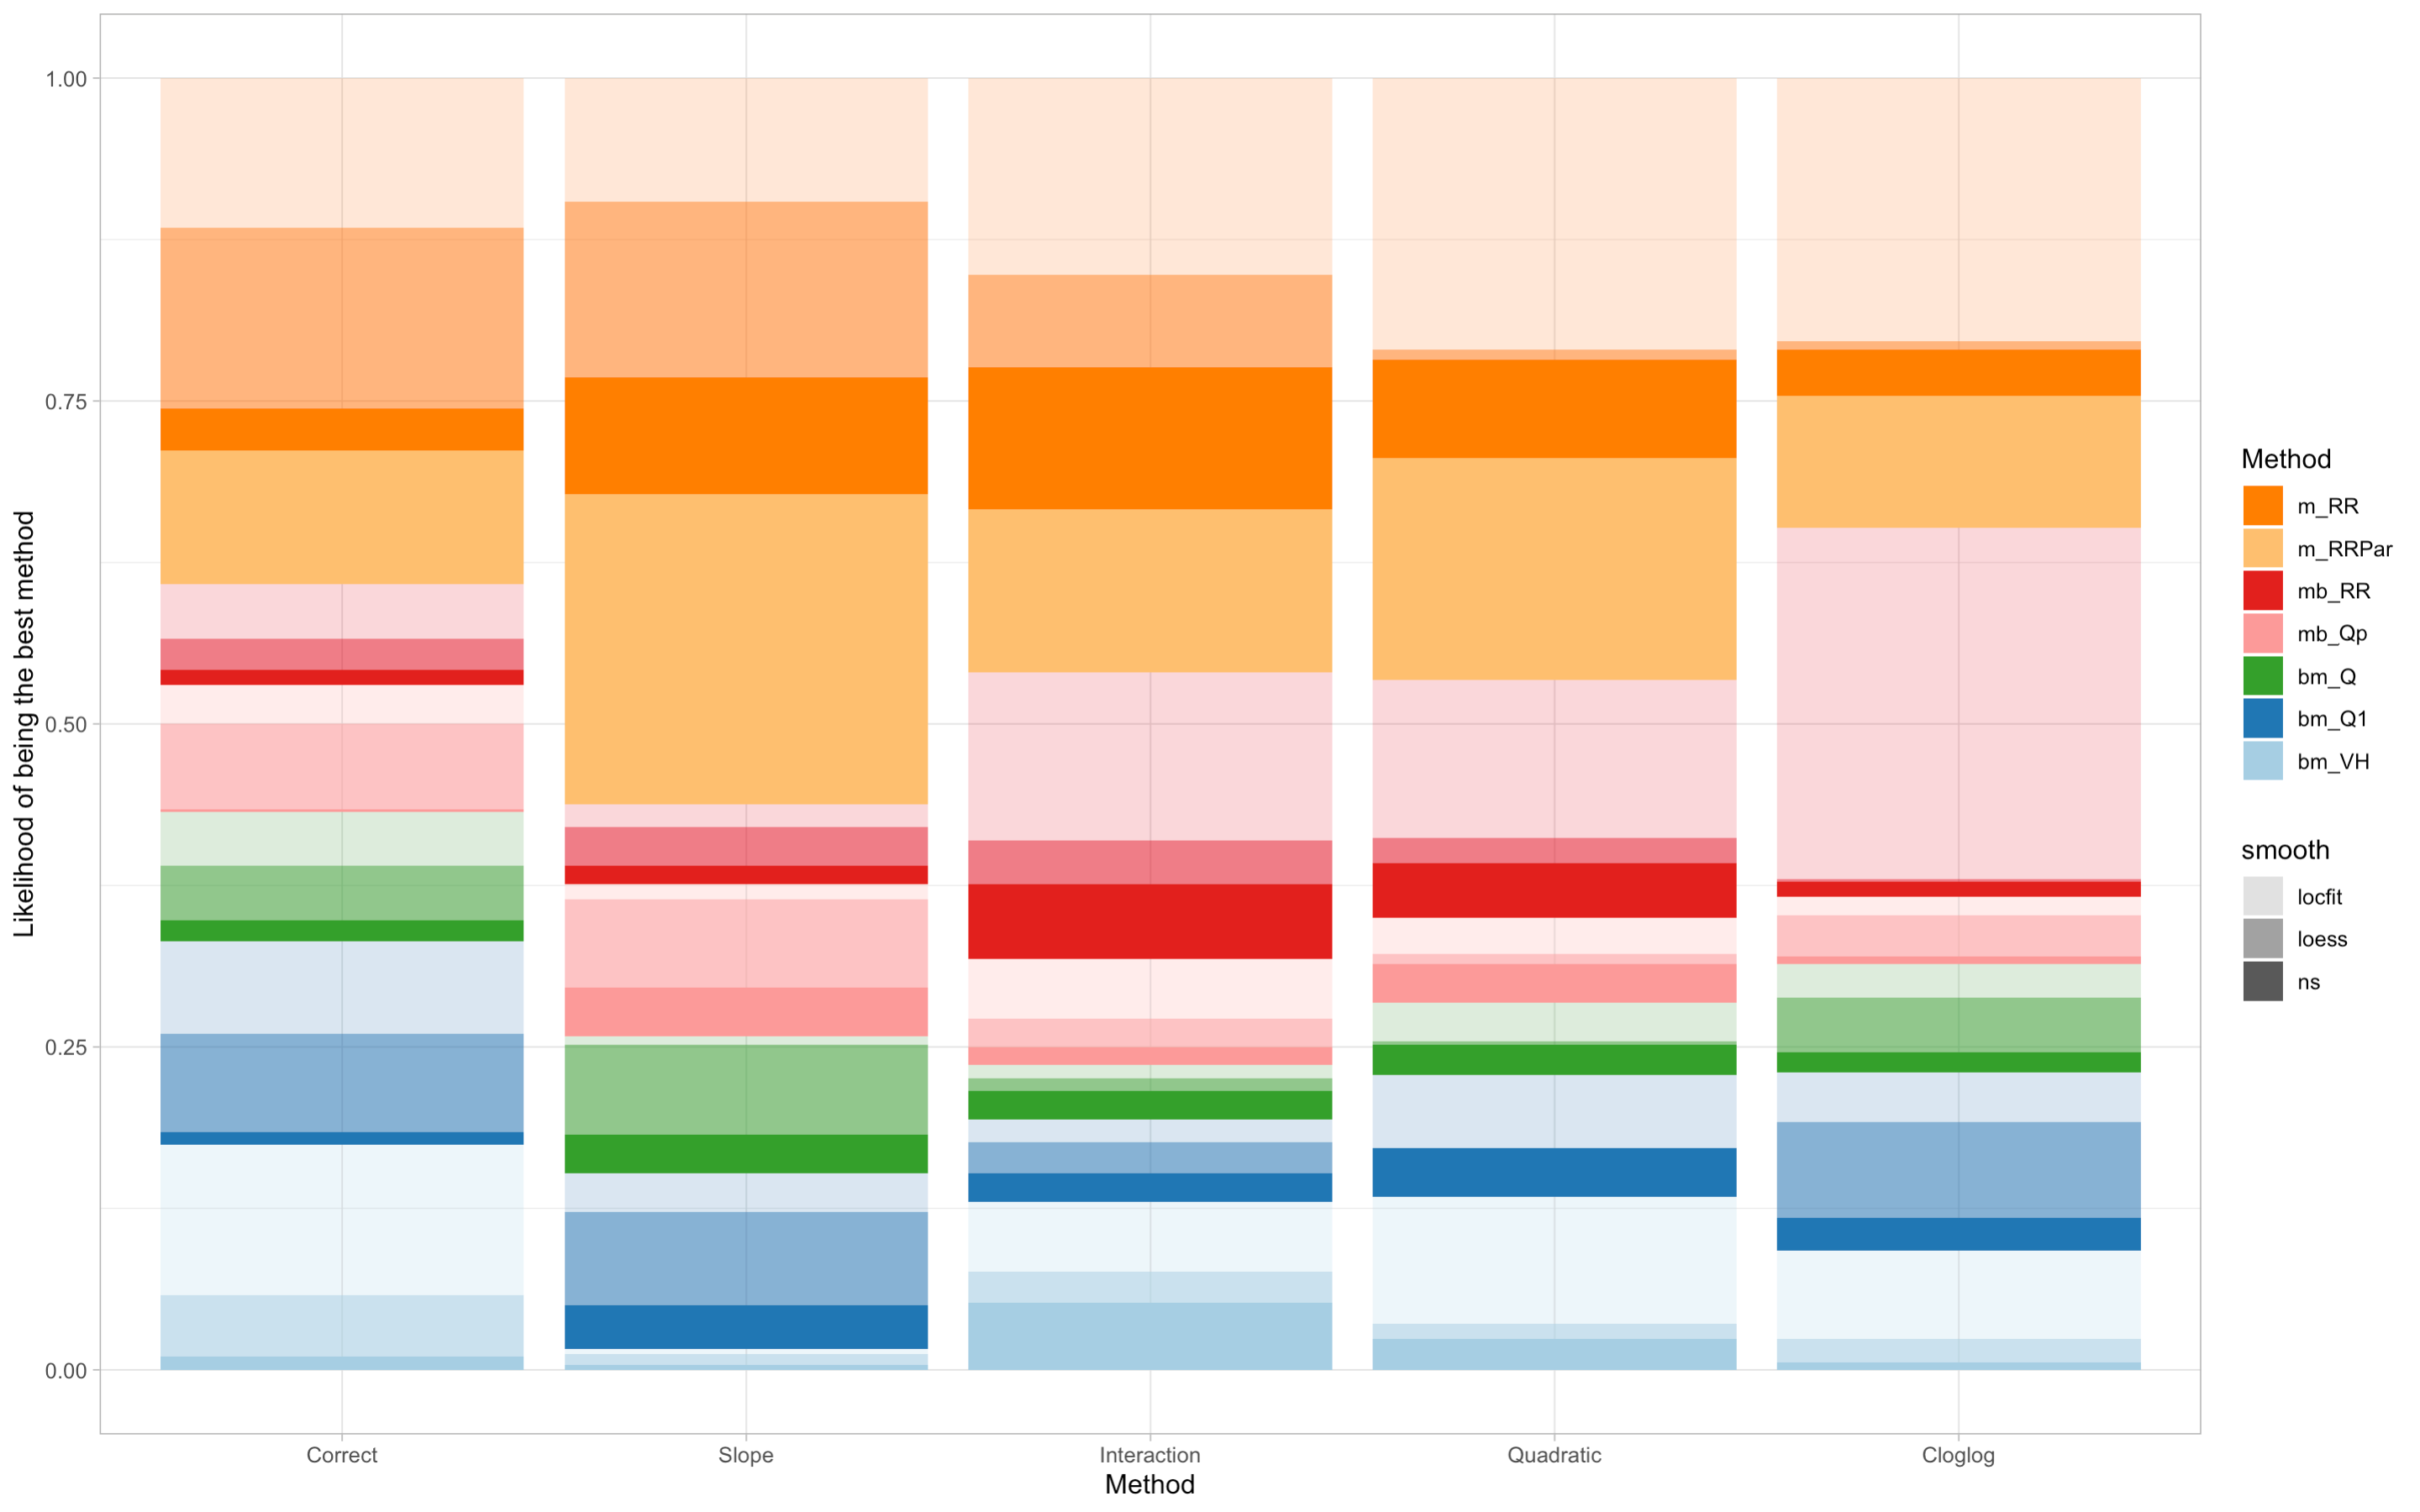
\includegraphics{images/probici.png}

\begin{center}\rule{0.5\linewidth}{0.5pt}\end{center}

{ Marginal results: Coverage} \includegraphics{images/medcov2.png}

\begin{center}\rule{0.5\linewidth}{0.5pt}\end{center}

{ Best method: Coverage} 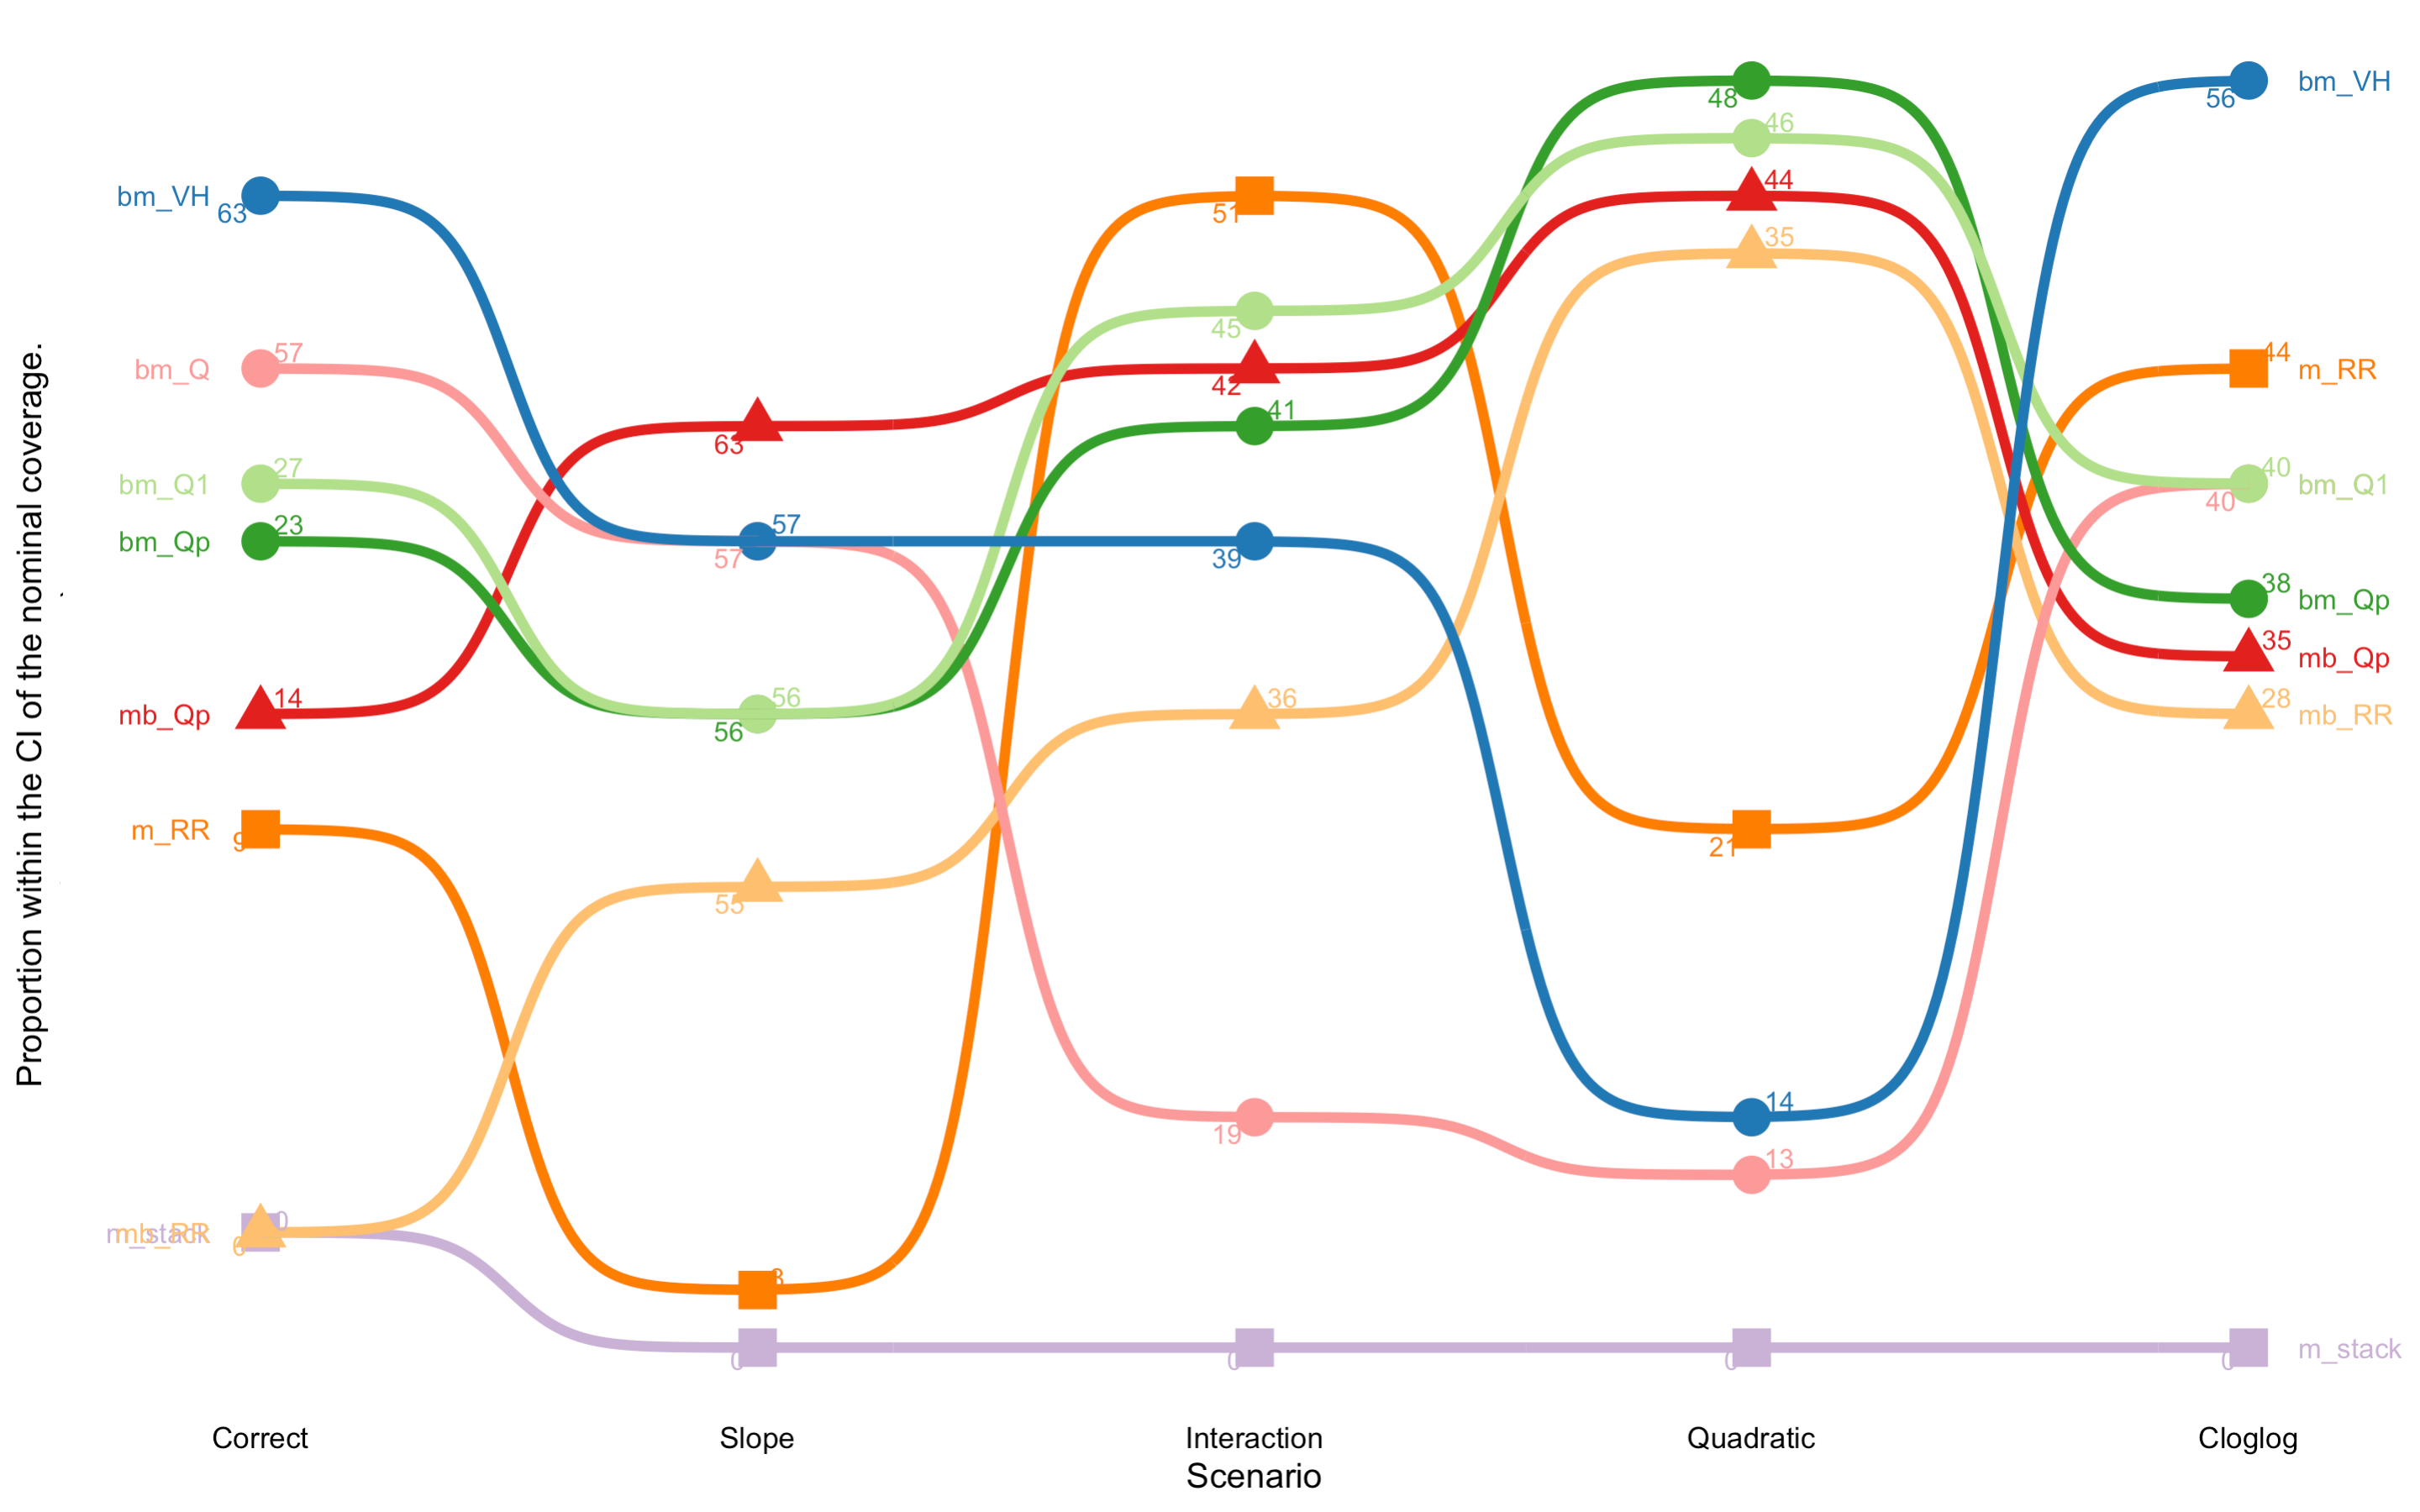
\includegraphics{images/rank.png} Proportion of
within 5\% of nominal coverage.

\begin{center}\rule{0.5\linewidth}{0.5pt}\end{center}

{ Conclusion}

\begin{itemize}
\item
  From the simulation, we could not find an overall winning method in
  terms of coverage and bias, but methods using bootstrap followed by
  MICE in general produce calibration curves with more proportion of
  points within 5\% of nominal coverage.
\item
  Considering processing time, a promising strategy could be Bootstrap
  with a single imputation method with a locfit smoother.
\end{itemize}

\begin{center}\rule{0.5\linewidth}{0.5pt}\end{center}

{ References}

\begin{enumerate}
\def\labelenumi{\arabic{enumi}.}
\tightlist
\item
  Austin PC, Steyerberg EW. Graphical assessment of internal and
  external calibration of logistic regression models by using loess
  smoothers. Stat Med. 2014; 33(3): 517-535.
\item
  Harrell FE Jr.~Regression Modeling Strategies. 2nd ed.~New York, NY:
  Springer-Verlag; 2015.
\item
  Bartlett, J. W., \& Hughes, R. A. (2020). Bootstrap inference for
  multiple imputation under uncongeniality and misspecification.
  Statistical methods in medical research, 29(12), 3533-3546.
\item
  Schomaker, M., \& Heumann, C. (2018). Bootstrap inference when using
  multiple imputation. Statistics in medicine, 37(14), 2252-2266.
\end{enumerate}

\begin{center}\rule{0.5\linewidth}{0.5pt}\end{center}



\end{document}
